\chapter{消息完整性}\label{chap:6}

在前几章中,我们重点讨论了针对窃听对手的安全性。窃听攻击的对手有能力窃听传输的消息,但不能在途中篡改这些消息。我们表明,选择明文安全是抵御这种攻击所需的自然安全属性。

在本章中,我们将注意力转向主动对手。我们从\emph{消息完整性}的基本问题开始。Bob 从 Alice 那里收到一条消息 $m$,并想确认这条消息在传输过程中没有遭到篡改。我们将会设计一个机制,它能让 Alice 为消息 $m$ 计算一个简短的消息完整性标签 $t$,并将这个数对 $(m,t)$ 发送给 Bob,如图 \ref{fig:6-1} 所示。Bob 在收到数对后会检查标签 $t$,如果检查未能通过,他就拒绝该消息。反之,如果验证通过,Bob 就能确信消息在传输途中并未遭到篡改。

需要强调的是,本章中的消息本身不需要是秘密的。和前几章不同,在本章中,我们的目标并不是隐藏信息。相反,我们只关注消息的完整性。在第\ref{chap:9}章中,我们还会讨论同时保证消息的机密性和完整性这一更普遍的问题。有许多应用需要保证消息的完整性,但并不要求机密性。我们举两个例子。

\begin{example}\label{exmp:6-1}
考虑一下通过互联网传递金融新闻或股票报价的问题。虽然新闻本身是公共信息,但至关重要的一点是,必须要确保没有第三方在消息发送给用户的过程中篡改数据。在这里,消息的机密性是无关紧要的,但完整性却非常关键。我们构造想要确保,如果用户 Bob 拒绝所有带有无效的消息完整性标签的消息,那么攻击者就不能注入看起来合法的修改内容。有一点需要注意的是,攻击者仍然可以改变新闻报道到达 Bob 的顺序。例如,Bob 可能在看到 $1$ 号报告之前看到 $2$ 号报告。在某些情况下,这可能导致用户采取错误的行动。为了防止这种情况,新闻服务可能需要在每份报告中包含一个序列号,以便用户的机器可以缓冲报告,并确保用户总是能以正确的顺序看到新闻。
\end{example}

在本章中,我们只关注试图修改数据的攻击。我们不考虑拒绝服务 (Denial of Service, DoS) 攻击,即攻击者迟滞或阻止新闻到达用户。防御 DoS 攻击的常用方法是确保从发送方到接收方的网络中存在冗余路径,这样攻击者就很难封锁所有路径。我们在本章中不会讨论这些问题。

\begin{example}\label{exmp:6-2}
考虑一个在磁盘上存储数据的应用程序,如文字处理机或者邮件客户端。尽管应用程序的代码并不是机密的(甚至在公共领域中),但其完整性至关重要。在运行该程序之前,用户希望确保存储在磁盘上的代码没有被病毒篡改。为此,在第一次安装程序时,用户为代码计算出一个信息完整性标签,并将该标签与程序一起存储在磁盘上。之后,在每次启动应用程序之前,用户需要验证这个消息完整性标签。如果该标签仍然是有效的,用户就可以确信,自从该标签最初被生成以来,代码没有被修改过。显然,病毒可以同时覆盖应用程序的代码和完整性标签。尽管如此,我们的构造将确保没有病毒可以欺骗用户运行未经认证的代码。就像我们在例 \ref{exmp:6-1} 中所述的那样,攻击者可以交换两个认证程序,当用户启动程序 $A$ 时,它就运行程序 $B$。对此的标准防御方法是在可执行文件中包含程序名称。这样,当一个应用程序被启动时,系统可以向用户显示一个经过验证的应用程序名称。
\end{example}

那么,问题就在于,如何设计一个安全的消息完整性机制?我们首先需要论证以下基本原则:
\begin{quote}
在两个通信方之间提供消息的完整性需要发送方有一个对手不知道的密钥。
\end{quote}
没有密钥,想要确保消息完整性就是不可能的,因为对手拥有足够的信息来计算它选择的任意消息的完整性标签——它知道消息完整性算法是如何工作的,这就足以用来计算标签了。因此,所有的密码学消息完整性机制都需要一个对手不知道的密钥。在本章中,我们将假设发送方和接收方都将共享秘钥;但在后面的章节中,我们还将进一步放宽这一假设。

需要强调的是,不是为安全性而设计的通信协议中经常使用\emph{无密钥}的完整性机制。例如,以太网协议使用 CRC32 作为其消息完整性算法。这个算法是公开的,它将输出的 $32$ 比特标签嵌入到每个以太网帧中。TCP 协议使用一个无密钥的 $16$ 比特校验和,它会被嵌入到每个数据包中。我们强调,这些无密钥的完整性机制是为了检测\emph{随机的}传输错误而设计的,并不能针对恶意的篡改。上一段的论证表明,对手可以很容易地攻破这些机制,并产生看起来合法的消息。例如,在以太网的场景中,对手完全知道 CRC32 算法的工作原理,这样它就可以计算出任意消息的有效标签。然后,它就可以篡改以太网流量而不被发现。

\begin{figure}
  \centering
%  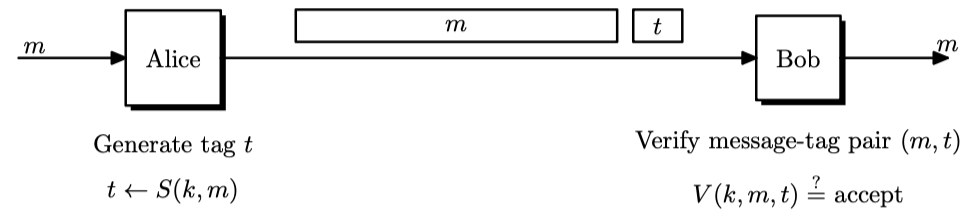
\includegraphics[width=0.75\linewidth]{figures/chapter6/fig1.png}
  \tikzset{every picture/.style={line width=0.75pt}}

\begin{tikzpicture}[x=0.75pt,y=0.75pt,yscale=-1,xscale=1]


\draw  [fill={rgb, 255:red, 255; green, 255; blue, 255 }  ,fill opacity=1 ][line width=1.2] [general shadow={fill=black,shadow xshift=2.25pt,shadow yshift=-2.25pt}] (60,0) -- (120,0) -- (120,60) -- (60,60) -- cycle ;
\draw  [fill={rgb, 255:red, 255; green, 255; blue, 255 }  ,fill opacity=1 ][line width=1.2] [general shadow={fill=black,shadow xshift=2.25pt,shadow yshift=-2.25pt}] (390,0) -- (450,0) -- (450,60) -- (390,60) -- cycle ;

\draw [line width=1.2]  (160,0) -- (310,0) -- (310,20) -- (160,20) -- cycle ;
\draw [line width=1.2]  (320,0) -- (350,0) -- (350,20) -- (320,20) -- cycle ;

\draw  [->]  (0,30) -- (59,30) ;
\draw  [->]  (120,30) -- (389,30) ;
\draw  [->]  (450,30) -- (510,30) ;

% Text Node
\draw (90,30) node   [align=left] {Alice};
% Text Node
\draw (2,26.6) node [anchor=south west] [inner sep=0.75pt]    {$m$};
% Text Node
\draw (502,26.6) node [anchor=south west] [inner sep=0.75pt]    {$m$};
% Text Node
\draw (235,10) node    {$m$};
% Text Node
\draw (335,10) node    {$t$};
% Text Node
\draw (420,30) node   [align=left] {Bob};
% Text Node
\draw (90,80) node   [align=left] {生成标签 $\displaystyle t$};
% Text Node
\draw (90,100) node    {$t\leftarrow S( k,m)$};
% Text Node
\draw (420,80) node   [align=left] {验证消息-标签对 $\displaystyle ( m,t)$};
% Text Node
\draw (420,100) node    {$V( k,m,t)\overset{?}{=}\mathsf{accept}$};


\end{tikzpicture}
  \caption{添加到消息上的短的消息完整性标签}
  \label{fig:6-1}
\end{figure}

\section{消息认证码的定义}\label{sec:6-1}

我们首先定义什么是基于发送方和接收方之间共享密钥的消息完整性系统。由于历史原因,这种系统被称为\textbf{消息认证码 (Message Authentication Code, MAC)}。

\begin{definition}\label{def:6-1}
一个 \textbf{MAC} 系统 $\mathcal{I}=(S,V)$ 是一对有效算法 $S$ 和 $V$,其中 $S$ 称为\textbf{签名算法 (signing algorithm)},$V$ 称为\textbf{验证算法 (verification algorithm)}。算法 $S$ 用于生成标签,算法 $V$ 用于验证标签。
\begin{itemize}
	\item $S$ 是一个概率性算法,其调用方式为 $t\overset{\rm R}\leftarrow S(k,m)$,其中 $k$ 是一个密钥,$m$ 是一条消息,输出 $t$ 称为\textbf{标签 (tag)}。
	\item $V$ 是一个确定性算法,其调用方式为 $r\leftarrow V(k,m,t)$,其中 $k$ 是一个密钥,$m$ 是一条消息,$t$ 是一个标签,输出 $r$ 是 $\mathsf{accept}$ 或者 $\mathsf{reject}$。
	\item 我们要求,由 $S$ 生成的标签总是会被 $V$ 接受;也就是说,MAC 必须满足以下\textbf{正确性属性 (correctness property)}:对于所有密钥 $k$ 和所有消息 $m$,都有:
\end{itemize}
\[
\Pr\left[V\big(k,\,m,\,S(k,m)\big)=\mathsf{accept}\right]=1
\]
和之前一样,我们说密钥位于某个有限的\textbf{密钥空间} $\mathcal{K}$ 中,消息位于一个有限的\textbf{消息空间} $\mathcal{M}$ 中,标签位于某个有限的\textbf{标签空间} $\mathcal{T}$ 中。我们称 $\mathcal{I}=(S,V)$ 定义在 $(\mathcal{K},\mathcal{M},\mathcal{T})$ 上。
\end{definition}

图 \ref{fig:6-1} 展示了算法 $S$ 和算法 $V$ 是如何保护双方的网络通信的。每当算法 $V$ 对某个消息-标签对 $(m,t)$ 输出 $\mathsf{accept}$ 时,我们就称 $t$ 是 $m$ 在密钥 $k$ 下的\textbf{有效标签 (valid tag)},或者说 $(m,t)$ 是 $k$ 下的\textbf{有效对 (valid pair)}。自然,我们希望 MAC 系统中的标签尽可能短,以使得传输标签的开销最小。

在本章中,我们将探索各种 MAC 系统。在最简单的 MAC 系统中,签名算法 $S$ 是确定性的,而验证算法的定义为:
\[
V(k,m,t)=\left\{
\begin{array}{ll}
\mathsf{accept}, & S(k,m)=t\\
\mathsf{reject}, & \text{otherwise}
\end{array}
\right.
\]
我们称这样的 MAC 系统为\textbf{确定性 MAC 系统}。确定性 MAC 系统的一个属性是它有\textbf{唯一标签 (unique tags)},即对于一个给定的密钥 $k$ 和一条给定的消息 $m$,该系统在 $k$ 下对 $m$ 有一个唯一的有效标签。不是所有的 MAC 系统都有这样简单的设计,有些可能会有随机的签名算法,所以对于给定的密钥 $k$ 和消息 $m$,$S(k,m)$ 的输出可能是许多可能的有效标签中的一个,而验证算法会以其他方式工作。正如我们将看到的,这种\textbf{随机化 MAC 系统}不是实现安全的必要条件,但它们可以产生更好的效率/安全权衡。

\begin{snote}[安全的 MAC。]
接下来,我们尝试描述一个 MAC 系统的安全性到底意味着什么。为了构建在各种应用中都能保持安全的 MAC,我们将坚持在一个非常恶劣的环境中定义安全性。由于大多数现实世界中使用 MAC 的系统都运行在不太恶劣的环境中,因此我们保守的安全定义将能够保证所有系统的安全性。

我们首先直观地解释这个定义,然后说明为什么这个保守的定义是有意义的。假设一个对手正在攻击一个 MAC 系统 $\mathcal{I}=(S,V)$。令 $k$ 是某个随机选出的 MAC 密钥,它对攻击者是未知的。我们允许攻击者为其选出的任意消息 $m$ 请求标签 $t:=S(k,m)$。这种攻击被称为\textbf{选择消息攻击 (chosen message attack)},它让攻击者能够收集到数以百万计的有效消息-标签对。显然,我们给了攻击者相当大的权力——很难想象一个用户会蠢到签署由攻击者提供的任意消息。然而,我们将看到,在现实世界的环境下,选择消息攻击时有出现。我们把对手使用选择消息攻击获得的信息-标签对 $(m,t)$ 称为\textbf{签名对 (signed pair)}。

使用选择消息攻击,我们要求攻击者给出一个\textbf{存在性 MAC 伪造 (existential MAC forgery)}。也就是说,攻击者只需要想出一些\emph{新的}有效信息-标签对 $(m,t)$。所谓``新",我们指的是与所有已有签名对都不同的消息-标签对。攻击者可以自由地选择 $m$;事实上,$m$ 不需要有任何特殊的格式或意义,甚至完全可以是胡言乱语。

如果一个能够发动选择消息攻击的对手也不能创造一个存在性 MAC 伪造,我们就称这个 MAC 系统是安全的。这个定义给对手的权力和空间比它在现实场景中能得到的要多得多,而且我们要求它做的也都是一些看起来没什么意义的事情;为一个没有意义的消息伪造 MAC 似乎是没有什么用处的。然而,正如我们将要看到的,这种保守的定义是非常自然的,它使我们能够将 MAC 用于许多不同的应用。

我们使用挑战者和对手 $\mathcal{A}$ 之间的一个攻击游戏来精确地定义一个安全的 MAC。下面的文字描述和图 \ref{fig:6-2} 共同刻画了这个攻击游戏。
\end{snote}

\begin{game}[MAC 的安全性]\label{game:6-1}
对于定义在 $(\mathcal{K},\mathcal{M},\mathcal{T})$ 上一个给定的 MAC 系统 $\mathcal{I}=(S,V)$,以及一个给定的对手 $\mathcal{A}$,攻击游戏运行如下:
\begin{itemize}
	\item 挑战者随机选取 $k\overset{\rm R}\leftarrow\mathcal{K}$。
	\item $\mathcal{A}$ 向挑战者发起多次查询。\\
	对于 $i=1,2,\dots$,第 $i$ 次\emph{签名查询}是一条消息 $m_i\in\mathcal{M}$。\\
	给定 $m_i$,挑战者计算出一个标签 $t_i\overset{\rm R}\leftarrow S(k,m_i)$,然后将 $t_i$ 交给 $\mathcal{A}$。
	\item 最终,$\mathcal{A}$ 输出一个不在签名对中的候选伪造对 $(m,t)\in\mathcal{M}\times\mathcal{T}$,即:
	\[(m,t)\notin\{(m_1,t_1),(m_2,t_2),\dots\}\]
\end{itemize}
如果 $(m,t)$ 是 $k$ 下的一个有效对(即 $V(k,m,t)=\mathsf{accept}$),我们就说 $\mathcal{A}$ 赢得了上述游戏。我们将 $\mathcal{A}$ 就 $\mathcal{I}$ 的优势表示为 ${\rm MAC}\mathsf{adv}[\mathcal{A},\mathcal{I}]$,即 $\mathcal{A}$ 赢得该游戏的概率。最后,如果 $\mathcal{A}$ 最多能够发起 $Q$ 次签名查询,我们就称 $\mathcal{A}$ 是一个 \textbf{$Q$ 次查询 MAC 对手}。
\end{game}

\begin{figure}
  \centering
%  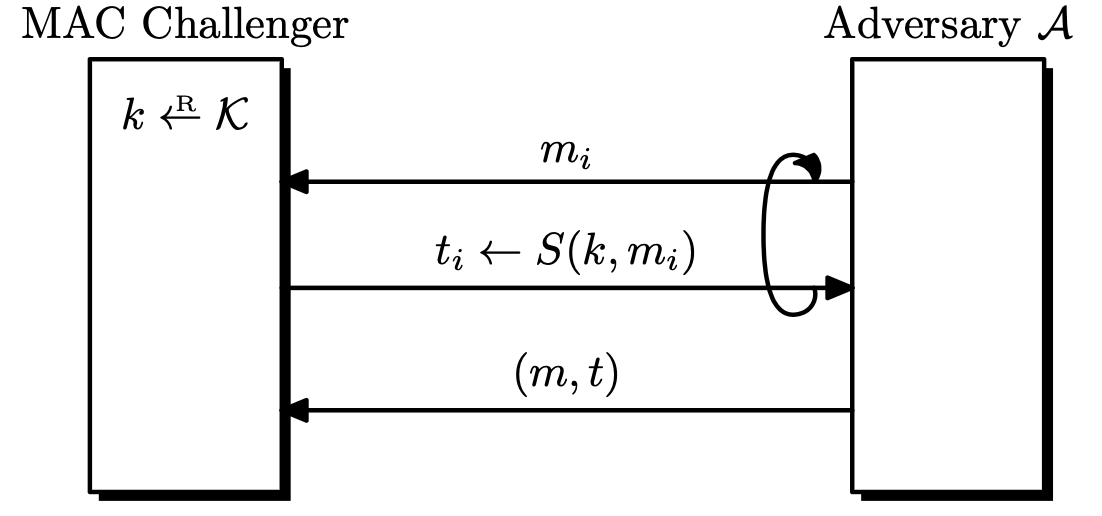
\includegraphics[width=0.5\linewidth]{figures/chapter6/fig2.png}
  \tikzset{every picture/.style={line width=0.75pt}} %set default line width to 0.75pt        

\begin{tikzpicture}[x=0.75pt,y=0.75pt,yscale=-1,xscale=1]
%uncomment if require: \path (0,195); %set diagram left start at 0, and has height of 195

%Shape: Rectangle [id:dp9400994371079527] 
\draw  [fill={rgb, 255:red, 255; green, 255; blue, 255 }  ,fill opacity=1 ][line width=1.2] [general shadow={fill=black,shadow xshift=2.25pt,shadow yshift=-2.25pt}] (30,30) -- (90,30) -- (90,180) -- (30,180) -- cycle ;
%Shape: Rectangle [id:dp23634228156893733] 
\draw  [fill={rgb, 255:red, 255; green, 255; blue, 255 }  ,fill opacity=1 ][line width=1.2] [general shadow={fill=black,shadow xshift=2.25pt,shadow yshift=-2.25pt}] (240,30) -- (300,30) -- (300,180) -- (240,180) -- cycle ;
%Straight Lines [id:da4832307524101793] 
\draw    (90,105) -- (237,105) ;
\draw [shift={(240,105)}, rotate = 180] [fill={rgb, 255:red, 0; green, 0; blue, 0 }  ][line width=0.08]  [draw opacity=0] (7.14,-3.43) -- (0,0) -- (7.14,3.43) -- cycle    ;
%Straight Lines [id:da49095779638687986] 
\draw    (95,140) -- (240,140) ;
\draw [shift={(92,140)}, rotate = 0] [fill={rgb, 255:red, 0; green, 0; blue, 0 }  ][line width=0.08]  [draw opacity=0] (7.14,-3.43) -- (0,0) -- (7.14,3.43) -- cycle    ;
%Straight Lines [id:da8544643220431498] 
\draw    (95,70) -- (240,70) ;
\draw [shift={(92,70)}, rotate = 0] [fill={rgb, 255:red, 0; green, 0; blue, 0 }  ][line width=0.08]  [draw opacity=0] (7.14,-3.43) -- (0,0) -- (7.14,3.43) -- cycle    ;
%Shape: Arc [id:dp898260212196978] 
\draw  [draw opacity=0] (231.07,104.86) .. controls (229.39,108.09) and (227.28,110) .. (225,110) .. controls (219.48,110) and (215,98.81) .. (215,85) .. controls (215,71.19) and (219.48,60) .. (225,60) .. controls (228.19,60) and (231.04,63.74) .. (232.87,69.56) -- (225,85) -- cycle ; \draw    (231.07,104.86) .. controls (229.39,108.09) and (227.28,110) .. (225,110) .. controls (219.48,110) and (215,98.81) .. (215,85) .. controls (215,71.19) and (219.48,60) .. (225,60) .. controls (227.65,60) and (230.06,62.58) .. (231.85,66.78) ; \draw [shift={(232.87,69.56)}, rotate = 245.45] [fill={rgb, 255:red, 0; green, 0; blue, 0 }  ][line width=0.08]  [draw opacity=0] (7.14,-3.43) -- (0,0) -- (7.14,3.43) -- cycle    ; 

% Text Node
\draw (60,45) node    {$k\overset{\mathrm{R}}{\leftarrow }\mathcal{K}$};
% Text Node
\draw (60,15) node   [align=left] {MAC 挑战者};
% Text Node
\draw (270,15) node   [align=left] {对手 $\displaystyle \mathcal{A}$};
% Text Node
\draw (166,66.6) node [anchor=south] [inner sep=0.75pt]    {$m_{i}$};
% Text Node
\draw (165,101.6) node [anchor=south] [inner sep=0.75pt]    {$t_{i}\leftarrow S( k,m_{i})$};
% Text Node
\draw (166,136.6) node [anchor=south] [inner sep=0.75pt]    {$( m,t)$};


\end{tikzpicture}
  \caption{MAC 攻击游戏(攻击游戏 \ref{game:6-1})}
  \label{fig:6-2}
\end{figure}

\begin{definition}\label{def:6-2}
如果对于所有有效对手 $\mathcal{A}$,${\rm MAC}\mathsf{adv}[\mathcal{A},\mathcal{I}]$ 的值都可忽略不计,我们就称 MAC 系统 $\mathcal{I}$ 是安全的。
\end{definition}

在对手赢得攻击游戏 \ref{game:6-1} 的情况下,它发送给挑战者的数对 $(m,t)$ 被称为\textbf{存在性伪造 (existential forgery)}。如果一个 MAC 系统满足定义 \ref{def:6-2},我们就称其在选择消息攻击下是\textbf{存在性不可伪造 (existential unforgeable)} 的。

在确定性 MAC 系统的情况下,$\mathcal{A}$ 赢得攻击游戏 \ref{game:6-1} 的唯一方法是为某个新消息 $m\notin\{m_1,m_2,\dots\}$  产生一个有效的消息-标签对 $(m,t)$。事实上,这种情况下的安全性只是意味着 $S$ 是\emph{不可预测的},参见 \ref{subsec:4-1-1} 小节给出的定义;也就是说,给定 $S(k,m_1),S(k,m_2),\dots$,对于任何 $m\notin\{m_1,m_2,\dots\}$,预测出 $S(k,m)$ 都是很难的。

在概率性 MAC 系统的情况下,我们的安全定义抓住了一个更强的属性。对于一条给定的消息,可能有许多条有效的标签。假设 $m$ 是某一条消息,又假设对手请求了 $m$ 的一条或多条有效标签 $t_1,t_2,\dots$,那么对手能否为 $m$ 产生一条新的有效标签 $t'$?(即一个满足 $t'\notin\{t_1,t_2,\dots\}$ 的标签)。我们的定义表明,对于一个有效对 $(m,t')$,如果 $t'$ 是新的,它就是一个有效的存在性伪造。因此,为了使 MAC 是安全的,对手必须很难为先前已经签署的消息 $m$ 产生一个新的有效标签 $t'$,这个对 MAC 的要求似乎很奇怪。如果对手已经有了 $m$ 的有效标签,我们为什么还要关心它是否能产生另一个呢?正如我们将要在第\ref{chap:9}章看到的,我们的安全定义,即防止对手在已签名的消息上产生新的标签,对于我们所考虑的应用是必要的。

回顾一下引言中的两个例子,我们可以发现,存在性不可伪造性意味着攻击者不能用一个有效标签来创建一条假的新闻报道。同样地,攻击者不能在篡改磁盘上程序的同时还不使程序的标签无效。但是,请注意,当使用 MAC 来保护应用程序的代码时,用户必须在每次要运行应用程序时提供他们的 MAC 密钥,这是一个很烦人的事情。在第\ref{chap:8}章,我们会讨论一种可以保护公共应用程序代码的无密钥方法。

为了深化对安全 MAC 的理解,我们不妨看几个案例。令 $\mathcal{I}=(S,V)$ 是一个定义在 $(\mathcal{K},\mathcal{M},\mathcal{T})$ 上的 MAC,令 $k$ 是 $\mathcal{K}$ 上的一个随机密钥。

\begin{example}\label{exmp:6-3}
假设 $m_1$ 和 $m_2$ 是几乎相同的两条消息。比如,$m_1$ 是一张 $100$ 美元的汇款单,而 $m_2$ 是一张 $101$ 美元的汇款单。显然,一个截获了 $m_1$ 的有效标签的对手不应当能够从中推导出$m_2$ 的有效标签。一个满足定义 \ref{def:6-2} 的 MAC 系统可以确保这一点。为了了解原因,假设一个对手 $\mathcal{A}$ 能够在给定 $m_1$ 的标签的情况下伪造 $m_2$ 的标签。那么,$\mathcal{A}$ 就可以赢得攻击游戏 \ref{game:6-1},方法是使用选择消息攻击来请求 $m_1$ 的标签,然后据此推导出 $m_2$ 的伪造标签 $t_2$,并输出 $(m_2,t_2)$ 作为有效的存在性伪造。显然,$\mathcal{A}$ 赢得了攻击游戏 \ref{game:6-1}。因此,存在性不可伪造性抓住了这样一个事实,即消息 $m_1$ 的标签对于产生另一条消息 $m_2$ 的标签来说不会提供任何有用的信息,即使 $m_2$ 和 $m_1$ 是几乎相同的。
\end{example}

\begin{example}\label{exmp:6-4}
我们对安全的 MAC 的定义使对手有能力获得任意消息的标签,这似乎是给了对手太多的权力。然而,在实践中,许多情况下,选择消息攻击是可行的。原因是 MAC 签名者往往不知道被签名数据的来源。例如,考虑一个将磁盘内容转储到备份磁带上的备份系统。由于备份的完整性是很重要的,系统为每一个将要被写入磁带的磁盘分组计算出一个完整性标签。该标签与数据分组一起被存储到磁带上。现在,假设一个攻击者将数据写到磁盘的低安全性区域。攻击者的数据将被备份,系统将对其计算出一个标签。通过检查所生成的备份磁带,攻击者就能获得它所选择的消息的标签。如果 MAC 系统对选择消息攻击是安全的,那么这种操作并不能帮助攻击者破解系统。
\end{example}

\begin{remark}\label{remark:6-1}
就像我们对其他安全原语所做的那样,我们可以把安全的 MAC 的概念推广到多密钥设置中,并证明一个安全的 MAC 在多密钥设置中也是安全的。参见练习 \ref{exer:6-3}。
\end{remark}

\subsection{数学细节}\label{subsec:6-1-1}

和之前一样,我们使用 \ref{sec:2-3} 节中定义的术语,对 MAC 给出一个更精确的数学定义。读者在初读时可以安全地跳过这一小节。

\begin{definition}[MAC]\label{def:6-3}
一个 \textbf{MAC} 系统是一对有效算法 $S$ 和 $V$,以及三个具有系统参数化 $P$ 的空间族:
\[
\mathbf{K}=\{\mathcal{K}_{\lambda,\Lambda}\}_{\lambda,\Lambda},\quad
\mathbf{M}=\{\mathcal{M}_{\lambda,\Lambda}\}_{\lambda,\Lambda},\quad
\mathbf{T}=\{\mathcal{T}_{\lambda,\Lambda}\}_{\lambda,\Lambda}
\]
和之前一样,$\lambda\in Z_{\geq1}$ 是一个安全参数,$\Lambda\in{\rm Supp}(P(\lambda))$ 是一个领域参数。我们要求:
\begin{enumerate}
	\item $\mathbf{K}$,$\mathbf{M}$ 和 $\mathbf{T}$ 是可有效识别的。
	\item $\mathbf{K}$ 是可有效采样的。
	\item 算法 $S$ 是一个有效的概率性算法,对于输入 $\lambda\in\mathbb{Z}_{\geq1}$,$\Lambda\in{\rm Supp}(P(\lambda))$,$k\in\mathcal{K}_{\lambda,\Lambda}$ 和 $m\in\mathcal{M}_{\lambda,\Lambda}$,$S$ 输出 $\mathcal{T}_{\lambda,\Lambda}$ 中的一个元素。
	\item 算法 $V$ 是一个有效确定性算法,对于输入 $\lambda\in\mathbb{Z}_{\geq1}$,$\Lambda\in{\rm Supp}(P(\lambda))$,$k\in\mathcal{K}_{\lambda,\Lambda}$,$m\in\mathcal{M}_{\lambda,\Lambda}$ 和 $t\in\mathcal{T}_{\lambda,\Lambda}$,$V$ 输出 $\mathsf{accept}$ 或 $\mathsf{reject}$。
\end{enumerate}

\end{definition}

在定义安全性时,我们通过安全参数 $\lambda$ 将攻击游戏 \ref{game:6-1} 参数化,对手和挑战者都会得到该参数。因此,优势 ${\rm MAC}\mathsf{adv}[\mathcal{A},\mathcal{I}]$ 也是 $\lambda$ 的一个函数。定义 \ref{def:6-2} 应该被理解为 ${\rm MAC}\mathsf{adv}[\mathcal{A},\mathcal{I}](\lambda)$ 是一个可忽略不计函数。
\section{MAC验证查询不会帮助攻击者}\label{sec:6-2}

在我们对安全的 MAC 的定义(攻击游戏 \ref{game:6-1})中,对手没有办法测试一个给定的信息-标签对是否有效。事实上,对手甚至无法判断它是否赢得了游戏,因为只有挑战者拥有运行验证算法所需的密钥。在现实生活中,一个有能力发动选择消息攻击的攻击者可能也能测试一个给定的消息-标签对是否有效。例如,攻击者可以建立一个有问题的消息-标签对数据包,并将它发送到受害者的机器上。然后,通过查看机器的行为,攻击者就可以知道该数据包是被接受了还是被丢弃了,进而确定该标签是否有效。

因此,通过赋予对手验证信息-标签对的额外权力来扩展攻击游戏 \ref{game:6-1} 是合理的。当然,我们仍然允许对手为它选择的任意消息请求标签。

\begin{game}[允许验证查询的 MAC 安全性]\label{game:6-2}
对于定义在 $(\mathcal{K},\mathcal{M},\mathcal{T})$ 上的一个给定的 MAC 系统 $\mathcal{I}=(S,V)$,以及一个给定的对手 $\mathcal{A}$,攻击游戏运行如下:
\begin{itemize}
	\item 挑战者随机选取 $k\overset{\rm R}\leftarrow\mathcal{K}$。
	\item $\mathcal{A}$ 向挑战者发起多次查询,每次查询可以是下面两种类型之一:
	\begin{itemize}
		\item \emph{签名查询}:对于 $i=1,2,\dots$,第 $i$ 次签名查询的内容是一条消息 $m_i\in\mathcal{M}$。挑战者计算出一个标签 $t_i\overset{\rm R}\leftarrow S(k,m_i)$,然后将 $t_i$ 交给 $\mathcal{A}$。
		\item \emph{验证查询}:对于 $j=1,2,\dots$,第 $j$ 次验证查询的内容是一个消息-标签对 $(\hat m_j,\hat t_j)\in\mathcal{M}\times\mathcal{T}$,该数对不在之前的签名对中,即:
		\[(\hat m_j,\hat t_j)\notin\{(m_1,t_1),(m_2,t_2),\dots\}\]
		挑战者将 $V(k,\hat m_j,\hat t_j)$ 发送给 $\mathcal{A}$。
	\end{itemize}
\end{itemize}
如果挑战者针对上述所有验证查询中的至少一个给出了 $\mathsf{accept}$ 的应答,我们就称 $\mathcal{A}$ 赢得了上述游戏。我们将 $\mathcal{A}$ 就 $\mathcal{I}$ 的优势表示为 ${\rm MAC^{vq}}\mathsf{adv}[\mathcal{A},\mathcal{I}]$,即 $\mathcal{A}$ 赢得该游戏的概率。
\end{game}

\begin{snote}[两个定义是等价的。]
攻击游戏 \ref{game:6-2} 在本质上与之前的攻击游戏 \ref{game:6-1} 是相同的,只是 $\mathcal{A}$ 可以发出 MAC 验证查询。我们证明,这种额外的权力并不能够帮助对手。
\end{snote}

\begin{theorem}\label{theo:6-1}
如果 $\mathcal{I}$ 是一个安全的 MAC 系统,那么它在存在验证查询的情况下也是安全的。
\begin{quote}
特别地,对于每个按照攻击游戏 \ref{game:6-2} 攻击 $\mathcal{I}$ 的 MAC 对手 $\mathcal{A}$,如果它最多能够发起 $Q_{\rm v}$ 次验证查询和 $Q_{\rm s}$ 次签名查询,则存在一个按照攻击游戏 \ref{game:6-1} 攻击 $\mathcal{I}$ 的 $Q_{\rm s}$ 次查询 MAC 对手 $\mathcal{B}$,其中 $\mathcal{B}$ 是一个围绕 $\mathcal{A}$ 的基本包装器,使得:
\end{quote}
\[
{\rm MAC^{vq}}\mathsf{adv}[\mathcal{A},\mathcal{I}]\leq{\rm MAC}\mathsf{adv}[\mathcal{A},\mathcal{I}]\cdot Q_{\rm v}
\]
\end{theorem}

\begin{proof}[证明思路]
假设 $\mathcal{A}$ 是一个 MAC 对手,它像攻击游戏 \ref{game:6-2} 中那样攻击 $\mathcal{I}$,并且最多进行 $Q_{\rm v}$ 次验证查询和 $Q_{\rm s}$ 次签名查询。我们可以基于对手 $\mathcal{A}$ 建立一个对手 $\mathcal{B}$,它如攻击游戏 \ref{game:6-1} 中那样攻击 $\mathcal{I}$,并最多进行 $Q_{\rm s}$ 次签名查询。对手 $\mathcal{B}$ 可以很容易地应答 $\mathcal{A}$ 的签名查询,只需要将这些查询转发给 $\mathcal{B}$ 的挑战者,并将挑战者产生的标签转发给 $\mathcal{A}$ 即可。

问题在于如何应答 $\mathcal{A}$ 的验证查询。根据定义,$\mathcal{A}$ 只会对不在之前已经签署的消息对中的消息提交验证查询。因此,$\mathcal{B}$ 可以采取一个简单的策略,即对 $\mathcal{A}$ 的所有验证查询都回复 $\mathsf{reject}$。如果 $\mathcal{B}$ 的回答是错的,它就得到了一个能够让它赢得攻击游戏 \ref{game:6-1} 的伪造消息。不幸的是,$\mathcal{B}$ 并不知道这些验证查询中的哪一个是伪造的,所以它只能猜测,也就是随机选择一个。由于 $\mathcal{A}$ 最多能发出 $Q_{\rm v}$ 次验证查询,所以 $\mathcal{B}$ 将以至少 ${1}/{Q_{\rm v}}$ 的概率猜对。这就是误差项中 $Q_{\rm v}$ 因子的来源。
\end{proof}

\begin{proof}
更详细地说,对手 $\mathcal{B}$ 在攻击游戏 \ref{game:6-2} 中扮演 $\mathcal{A}$ 的挑战者,同时在攻击游戏 \ref{game:6-1} 中扮演对手,并与该游戏中的 MAC 挑战者交互。它的工作逻辑如下:

\vspace{5pt}

\hspace*{5pt} 初始化:\\
\hspace*{50pt} 选取 $\omega\overset{\rm R}\leftarrow\{1,\dots,Q_{\rm v}\}$\\
\hspace*{26pt} 当从 $\mathcal{A}$ 处收到签名查询 $m_i\in\mathcal{M}$ 时:\\
\hspace*{50pt} 将 $m_i$ 转发给 MAC 挑战者,并获得标签 $t_i$\\
\hspace*{50pt} 将 $t_i$ 发送给 $\mathcal{A}$\\
\hspace*{26pt} 当从 $\mathcal{A}$ 处收到的验证查询 $(\hat m_j,\hat t_j)\in\mathcal{M}\times\mathcal{T}$ 时:\\
\hspace*{50pt} 如果 $j=\omega$:\\
\hspace*{75pt} 输出 $(\hat m_j,\hat t_j)$ 作为一个候选的伪造对,然后停机\\
\hspace*{50pt} 否则:\\
\hspace*{75pt} 向 $\mathcal{A}$ 发送 $\mathsf{reject}$

\vspace{5pt}

为了严格论证对手 $\mathcal{B}$ 的构造,我们分析 $\mathcal{A}$ 在以下三个密切相关的游戏中的行为。

\vspace{5pt}

\noindent\textbf{游戏$\mathbf{0}$}。
这是原始的攻击游戏,就如攻击游戏 \ref{game:6-2} 中 $\mathcal{A}$ 与挑战者之间进行的游戏一样。挑战者在该游戏中的逻辑如下:

\vspace{5pt}

\hspace*{5pt} 初始化:\\
\hspace*{50pt} 选取 $k\overset{\rm R}\leftarrow\mathcal{K}$\\
\hspace*{26pt} 当从 $\mathcal{A}$ 处收到签名查询 $m_i\in\mathcal{M}$ 时:\\
\hspace*{50pt} 令 $t_i\overset{\rm R}\leftarrow S(k,m_i)$\\
\hspace*{50pt} 将 $t_i$ 发送给 $\mathcal{A}$\\
\hspace*{26pt} 当从 $\mathcal{A}$ 处收到的验证查询 $(\hat m_j,\hat t_j)\in\mathcal{M}\times\mathcal{T}$ 时:\\
\hspace*{50pt} 令 $r_j\leftarrow V(k,\hat m_j,\hat t_j)$\\
\hspace*{10pt} ($*$)
\hspace*{19.5pt} 将 $r_j$ 发送给 $\mathcal{A}$

\vspace{5pt}


记 $W_0$ 为在游戏 $0$ 中,存在某个 $j$ 使得 $r_j=\mathsf{accept}$ 的事件。显然:
\begin{equation}\label{eq:6-1}
\Pr[W_0]={\rm MAC^{vq}}\mathsf{adv}[\mathcal{A},\mathcal{I}]
\end{equation}

\noindent\textbf{游戏$\mathbf{1}$}。
游戏 $1$ 与游戏 $0$ 基本相同,只是将游戏 $0$ 中标有 ($*$) 的一行改为:

\vspace{5pt}

\hspace*{50pt} 将 $\mathsf{reject}$ 发送给 $\mathcal{A}$

\vspace{5pt}

也就是说,在游戏 $1$ 中,在应答验证查询时,挑战者总是用 $\mathsf{reject}$ 来回应 $\mathcal{A}$。我们定义 $W_1$ 为在游戏 $1$ 中,存在某个 $j$ 使得 $r_j=\mathsf{accept}$ 的事件。尽管在游戏 $1$ 中,挑战者不会通知 $\mathcal{A}$ 事件 $W_1$ 发生了,但是在这个事件发生之前,游戏 $0$ 和游戏 $1$ 的进程事实上都是完全相同的,因此事件 $W_0$ 和 $W_1$ 在本质上是相同的,因此:
\begin{equation}\label{eq:6-2}
\Pr[W_1]=\Pr[W_0]
\end{equation}
此外,注意到,在游戏 $1$ 中,尽管 $r_j$ 被用来定义获胜的条件,但它们并没有被用于任何其他目的,因此不会以任何方式影响攻击。

\vspace{5pt}

\noindent\textbf{游戏$\mathbf{2}$}。
游戏 $2$ 与游戏 $1$ 基本相同,只是在游戏开始时,挑战者随机选取 $\omega\overset{\rm R}\leftarrow\{1,\dots,Q_{\rm v}\}$。我们定义 $W_2$ 为游戏 $2$ 中 $r_\omega=\mathsf{accept}$ 成立的事件。由于 $\omega$ 的选择与攻击本身无关,我们有:
\begin{equation}\label{eq:6-3}
\Pr[W_2]\geq{\Pr[W_1]}/{Q_{\rm v}}
\end{equation}

显然,根据构造,我们有:
\begin{equation}\label{eq:6-4}
\Pr[W_2]={\rm MAC}\mathsf{adv}[\mathcal{B},\mathcal{I}]
\end{equation}
于是,根据式 \ref{eq:6-1},\ref{eq:6-2} 和 \ref{eq:6-3},我们就能得到该定理成立。
\end{proof}

综上所述,我们表明,给予对手更多权力的攻击游戏 \ref{game:6-2} 和定义安全的 MAC 时使用的攻击游戏 \ref{game:6-1} 是等价的。这种归约在误差项中引入了一个 $Q_{\rm v}$ 的系数。在本书中,我们将使用这两个攻击游戏:
\begin{itemize}
	\item 当构建安全的 MAC 时,使用攻击游戏 \ref{game:6-1} 更容易,它限制对手只能发起签名查询。这使得我们更容易证明安全性,因为我们只需要考虑一种类型的查询。我们将在整个章节中使用这个攻击游戏。
	\item 当使用安全的 MAC 来构建更高层次的系统(如验证式加密)时,假设 MAC 对于攻击游戏 \ref{game:6-2} 中描述的更强的对手是安全的,是更方便的。
\end{itemize}

我们还指出,如果我们使用一个较弱的安全概念,即对手只通过在新消息上给出一个有效标签(而不是新的有效的消息-标签对)而获胜,那么攻击游戏 \ref{game:6-1} 和攻击游戏 \ref{game:6-2} 的类比就\emph{不}等价了(见练习 6.7)。
\section{使用 PRF 构建 MAC}\label{sec:6-3}

我们下面尝试使用我们已经掌握的工具来构建安全的 MAC。在前几章中,我们使用伪随机函数 (PRF) 来构建各种加密系统。我们举了一些实际的 PRF 的例子,比如 AES(虽然 AES 是一个分组密码,但由于 PRF 切换引理,即定理 \ref{theo:4-4},我们也可将其看作是一个 PRF)。在这里,我们表明,任何安全的 PRF 都可以直接被用来建立一个安全的 MAC。

回顾一下,PRF 是这样的一种算法 $F$,它接受密钥 $k$ 和数据分组 $x$ 作为输入,并输出一个值 $y:=F(k,x)$。通常,如果密钥在 $\mathcal{K}$ 上,输入在 $\mathcal{X}$ 上,输出在 $\mathcal{Y}$ 上,我们就称 $F$ 定义在 $(\mathcal{K},\mathcal{X},\mathcal{Y})$ 上。对于一个 PRF $F$,我们将\textbf{由 $F$ 派生出的确定性 MAC 系统} $\mathcal{I}=(S,V)$ 定义为:

\vspace{5pt}

\hspace*{5pt} $S(k,m)=F(k,m)$;

\vspace{5pt}

\hspace*{5pt} $
V(k,m,t)=\left\{
\begin{array}{ll}
\mathsf{accept}, & F(k,m)=t\\
\mathsf{reject}, & \text{otherwise}
\end{array}
\right.
$

\vspace{8pt}

正如已经讨论过的,任何具有大的(即超多项式的)输出空间的 PRF 都是不可预测的(见 \ref{subsec:4-1-1} 小节),因此,正如 \ref{sec:6-1} 节所讨论的,上述构造产生了一个安全的 MAC。完整起见,我们下面用一个定理来说明这一点。

\begin{theorem}\label{theo:6-2}
令 $F$ 是一个定义在 $(\mathcal{K},\mathcal{X},\mathcal{Y})$ 上的安全的 PRF,其中 $|\mathcal{Y}|$ 是超多项式的。那么,由 $F$ 派生的确定性 MAC 系统 $\mathcal{I}$ 是一个安全的 MAC。
\begin{quote}
特别地,对于每个按照攻击游戏 \ref{game:6-1} 攻击 $\mathcal{I}$ 的 $Q$ 次查询 MAC 对手 $\mathcal{A}$,都存在一个按照攻击游戏 \ref{game:4-2} 攻击 $F$ 的 $(Q+1)$ 次查询 PRF 对手 $\mathcal{B}$,其中 $\mathcal{B}$ 是一个围绕 $\mathcal{A}$ 的基本包装器,满足:
\end{quote}
\[
{\rm MAC}\mathsf{adv}[\mathcal{A},\mathcal{I}]\leq{\rm PRF\mathsf{adv}}[\mathcal{B}, F]+{1}/{|\mathcal{Y}|}
\]
\end{theorem}

\begin{proof}[证明思路]
令 $\mathcal{A}$ 是一个有效 MAC 对手。我们通过约束 $\mathcal{A}$ 产生伪造的信息-标签对的能力,推导出 ${\rm MAC}\mathsf{adv}[\mathcal{A},\mathcal{I}]$ 的上界。和之前一样,用 ${\rm Funs}[\mathcal{X},\mathcal{Y}]$ 中的一个真随机函数 $f$ 替换底层的安全 PRF $F$ 并不会使 $\mathcal{A}$ 的优势发生很大的变化。但是,如果对手 $\mathcal{A}$ 交互的对象是一个真随机函数,它将会面临一个没有希望的任务:它需要在它选定的几个点上获取 $f$ 的值,并发动选择消息攻击。然后,它需要猜测 $f(m)\in\mathcal{Y}$ 在某个新的点 $m$ 处的值。但由于 $f$ 是一个真随机函数,$\mathcal{A}$ 没有办法获得任何关于 $f(m)$ 的信息,因此它猜中 $f(m)$ 的概率微乎其微。
\end{proof}

\begin{proof}
我们通过让 $\mathcal{A}$ 与两个密切相关的挑战者交互来证明这个结论。

\vspace{5pt}

\noindent\textbf{游戏$\mathbf{0}$}。
和之前一样,我们先回顾 MAC 攻击游戏 \ref{game:6-1} 中的挑战者,它此时被应用于 $\mathcal{I}$。在这个游戏中,挑战者的逻辑如下:

\vspace{5pt}

\hspace*{-16.5pt} ($*$)
\hspace*{1pt} 选取 $k\overset{\rm R}\leftarrow\mathcal{K}$,令 $f\leftarrow F(k,\cdot)$\\
\hspace*{26pt} 当收到第 $i$ 个签名查询 $m_i\in\mathcal{M}$ ($i=1,2,\dots$) 时:\\
\hspace*{50pt} 令 $t_i\leftarrow f(m_i)$\\
\hspace*{50pt} 将 $t_i$ 发送给对手

\vspace{5pt}

\noindent
在游戏结束时,对手输出一个消息-标签对 $(m,t)$。我们将 $W_0$ 定义为条件:
\begin{equation}\label{eq:6-5}
t=f(m)
\quad\quad\text{and}\quad\quad
m\notin\{m_1,m_2,\dots\}
\end{equation}
在游戏 $0$ 中成立的事件。显然,$\Pr[W_0]={\rm MAC}\mathsf{adv}[\mathcal{A},\mathcal{I}]$ 成立。

\vspace{5pt}

\noindent\textbf{游戏$\mathbf{1}$}。
接下来,和之前一样,我们打出``PRF牌",用 ${\rm Funs}[\mathcal{X},\mathcal{Y}]$ 中的一个真随机函数 $f$ 替换 $F(k,\cdot)$。直观地说,由于 $F$ 是一个安全的 PRF,对手 $\mathcal{A}$ 应该不会注意到这种差别。游戏 $1$ 中的挑战者与游戏 $0$ 中的挑战者大致相同,只是我们将标有 ($*$) 的那一行改为:

\vspace{5pt}

\hspace*{-16.5pt} ($*$)
\hspace*{1pt} 选取 $f\overset{\rm R}\leftarrow{\rm Funs}[\mathcal{X},\mathcal{Y}]$

\vspace{5pt}

\noindent
令 $W_1$ 为式 \ref{eq:6-5} 在游戏 $1$ 中成立的事件。我们构建一个 $(Q+1)$ 次查询 PRF 对手 $\mathcal{B}$,满足:
\begin{equation}\label{eq:6-6}
|\Pr[W_1]-\Pr[W_0]|={\rm PRF}\mathsf{adv}[\mathcal{B},F]
\end{equation}
对手 $\mathcal{B}$ 通过查询自己的 PRF 挑战者来应答 $\mathcal{A}$ 的选择消息查询。最终,$\mathcal{A}$ 会输出一个候选的 MAC 伪造 $(m,t)$,其中 $m$ 不在 $\mathcal{A}$ 之前的选择信息查询中。现在,$\mathcal{B}$ 在 $m$ 处向它的 PRF 挑战者发起查询,并得到某个 $t'\in\mathcal{Y}$。如果 $t=t'$,$\mathcal{B}$ 就输出 $0$,否则就输出 $1$。不难证明,这样的对手 $\mathcal{B}$ 满足式 \ref{eq:6-6}。

接下来我们直接约束 $\Pr[W_1]$。对手 $\mathcal{A}$ 得到了 $f$ 在 $m_1,m_2,\dots$ 处的值,然后被要求猜测 $f$ 在一个新点 $m$ 处的值。但由于 $f$ 是一个真随机函数,所以值 $f(m)$ 与它在其他点处的值都无关。由于 $m\notin\{m_1,m_2,\dots\}$,所以对手 $\mathcal{A}$ 将以 ${1}/{|\mathcal{Y}|}$ 的概率猜中 $f(m)$。因此,$\Pr[W_1]\leq{1}/{|\mathcal{Y}|}$。将此与式 \ref{eq:6-6} 结合,我们可以得到:
\[
{\rm MAC}\mathsf{adv}[\mathcal{A},\mathcal{I}]
=\Pr[W_0]
\leq\big\lvert\Pr[W_0]−\Pr[W_1]\big\rvert+\Pr[W_1]
\leq{\rm PRF}\mathsf{adv}[\mathcal{B},F]+\frac{1}{|\mathcal{Y}|}
\]
因此本定理得证。
\end{proof}

\begin{snote}[具体的标签长度。]
该定理表明,为确保 ${\rm MAC}\mathsf{adv}[\mathcal{A},\mathcal{I}]<2^{128}$,我们需要这样的一个 PRF,其输出空间 $\mathcal{Y}$ 满足 $|\mathcal{Y}|>2^{128}$。如果输出空间 $\mathcal{Y}$ 形如 $\{0,1\}^n$,其中 $n$ 是某个整数,那么产生的标签至少长 $128$ 比特。
\end{snote}
\section{用于长消息的无前缀PRF}\label{sec:6-4}

在上一节中,我们看到,任何一个安全的 PRF 也是一个安全的 MAC。然而,第\ref{chap:4}章中的 PRF 实例只接受短的输入,因而只能为非常短的消息提供完整性。比如,如果将 AES 看作是一个 PRF,我们就能得到一个用于 $128$ 比特消息的 MAC。现在,我们想要为更长的消息构建 MAC。

本章中所有的 MAC 构造都遵循同样的范式:它们从短输入的 PRF 开始(如 AES),产生一个 PRF,继而构造一个能用于更长输入的 MAC。因此,我们在本章的剩余部分的目标如下:
\begin{quote}
\textbf{给定一个针对短消息输入的安全 PRF,构建一个针对长消息输入的安全 PRF。}
\end{quote}
我们将会分三步来解决这个问题:
\begin{itemize}
	\item 首先,在本节中,我们为长输入构建\emph{无前缀安全的 PRF}。更确切地说,给定一个在单分组(比如 $128$ 比特)上运行的安全 PRF,我们想要构建一个无前缀的安全 PRF。回顾一下,无前缀安全 PRF(定义 \ref{def:4-5})只在有限的意义上是安全的:我们只要求\emph{无前缀对手}无法区分 PRF 和随机函数。一个无前缀 PRF 对手发出的查询是非空的分组序列,且其中的任何一个查询都不是其他查询的真前缀。
	\item 其次,在接下来的几节中,我们将展示如何把用于长输入的无前缀安全 PRF 转换成用于长输入的完全安全 PRF。因此,在这几节结束时,我们将得到几个这样的安全 PRF,并由此构造出能够用于长消息的安全的 MAC。
	\item 第三,在 \ref{sec:6-8} 节中,我们将展示,如何将一个作用于由分组序列构成的消息的 PRF 转换为一个作用于比特序列的 PRF。
\end{itemize}

\begin{snote}[无前缀的 PRF。]
我们从两个经典的无前缀安全 PRF 构造开始。图 \ref{fig:6-3-a} 展示了 \textbf{CBC} 构造,图 \ref{fig:6-3-b} 展示了\textbf{级联}构造。我们表明,当底层函数 $F$ 是一个安全的 PRF 时,CBC 构造和级联构造都是无前缀安全的 PRF。
\end{snote}

\begin{figure}
  \centering
  \subfigure[CBC构造$F_\mathrm{CBC}(k,m)$]{
    \tikzset{every picture/.style={line width=0.75pt}}

\begin{tikzpicture}[x=0.75pt,y=0.75pt,yscale=-1,xscale=1]

\draw  [fill={rgb, 255:red, 255; green, 255; blue, 255 }  ,fill opacity=1 ][line width=1.2] [general shadow={fill=black,shadow xshift=2.25pt,shadow yshift=-2.25pt}] (10,90) -- (60,90) -- (60,140) -- (10,140) -- cycle ;
\draw  [fill={rgb, 255:red, 255; green, 255; blue, 255 }  ,fill opacity=1 ][line width=1.2] [general shadow={fill=black,shadow xshift=2.25pt,shadow yshift=-2.25pt}] (0,0) -- (70,0) -- (70,20) -- (0,20) -- cycle ;
\draw  [fill={rgb, 255:red, 255; green, 255; blue, 255 }  ,fill opacity=1 ][line width=1.2] [general shadow={fill=black,shadow xshift=2.25pt,shadow yshift=-2.25pt}] (100,0) -- (170,0) -- (170,20) -- (100,20) -- cycle ;
\draw  [fill={rgb, 255:red, 255; green, 255; blue, 255 }  ,fill opacity=1 ][line width=1.2] [general shadow={fill=black,shadow xshift=2.25pt,shadow yshift=-2.25pt}] (200,0) -- (270,0) -- (270,20) -- (200,20) -- cycle ;
\draw  [fill={rgb, 255:red, 255; green, 255; blue, 255 }  ,fill opacity=1 ][line width=1.2] [general shadow={fill=black,shadow xshift=2.25pt,shadow yshift=-2.25pt}] (330,0) -- (400,0) -- (400,20) -- (330,20) -- cycle ;
\draw  [fill={rgb, 255:red, 255; green, 255; blue, 255 }  ,fill opacity=1 ][line width=1.2] [general shadow={fill=black,shadow xshift=2.25pt,shadow yshift=-2.25pt}] (110,90) -- (160,90) -- (160,140) -- (110,140) -- cycle ;
\draw  [fill={rgb, 255:red, 255; green, 255; blue, 255 }  ,fill opacity=1 ][line width=1.2] [general shadow={fill=black,shadow xshift=2.25pt,shadow yshift=-2.25pt}] (210,90) -- (260,90) -- (260,140) -- (210,140) -- cycle ;
\draw  [fill={rgb, 255:red, 255; green, 255; blue, 255 }  ,fill opacity=1 ][line width=1.2] [general shadow={fill=black,shadow xshift=2.25pt,shadow yshift=-2.25pt}] (340,90) -- (390,90) -- (390,140) -- (340,140) -- cycle ;

\draw  [->]  (35,20) -- (35,90) ;
\draw  [->]  (60,115) -- (85,115) -- (85,55) -- (130,55) ;
\draw  [->]  (160,115) -- (185,115) -- (185,55) -- (230,55) ;
\draw  [->]  (330,55) -- (360,55) ;
\draw  [->]  (135,20) -- (135,50) ;
\draw  [->]  (135,60) -- (135,90) ;
\draw  [->]  (235,20) -- (235,50) ;
\draw  [->]  (365,20) -- (365,50) ;
\draw  [->]  (235,60) -- (235,90) ;
\draw  [->]  (365,60) -- (365,90) ;
\draw  [->]  (260,115) -- (285,115) ;
\draw  [->]  (390,115) -- (440,115) ;

\draw  [dash pattern={on 0.84pt off 2.51pt}]  (285,115) -- (310,115) -- (310,55) -- (330,55) ;


% Text Node
\draw (35,115) node    {$F( k,\cdot )$};
% Text Node
\draw (135,115) node    {$F( k,\cdot )$};
% Text Node
\draw (235,115) node    {$F( k,\cdot )$};
% Text Node
\draw (365,115) node    {$F( k,\cdot )$};
% Text Node
\draw (135,55) node  [font=\large]  {$\oplus $};
% Text Node
\draw (235,55) node  [font=\large]  {$\oplus $};
% Text Node
\draw (365,55) node  [font=\large]  {$\oplus $};
% Text Node
\draw (300,10) node    {$\cdots $};
% Text Node
\draw (35,10) node    {$a_{1}$};
% Text Node
\draw (135,10) node    {$a_{2}$};
% Text Node
\draw (235,10) node    {$a_{3}$};
% Text Node
\draw (365,10) node    {$a_{\ell }$};
% Text Node
\draw (440,111.6) node [anchor=south] [inner sep=0.75pt]    {$tag$};


\end{tikzpicture}
  	\label{fig:6-3-a}
  }
  
  \,
  
  \,
  
  \subfigure[级联构造$F^*(k,m)$]{
  	\tikzset{every picture/.style={line width=0.75pt}}

\begin{tikzpicture}[x=0.75pt,y=0.75pt,yscale=-1,xscale=1]

\draw  [fill={rgb, 255:red, 255; green, 255; blue, 255 }  ,fill opacity=1 ][line width=1.2] [general shadow={fill=black,shadow xshift=2.25pt,shadow yshift=-2.25pt}] (50,50) -- (100,50) -- (100,100) -- (50,100) -- cycle ;
\draw  [fill={rgb, 255:red, 255; green, 255; blue, 255 }  ,fill opacity=1 ][line width=1.2] [general shadow={fill=black,shadow xshift=2.25pt,shadow yshift=-2.25pt}] (40,0) -- (110,0) -- (110,20) -- (40,20) -- cycle ;
\draw  [fill={rgb, 255:red, 255; green, 255; blue, 255 }  ,fill opacity=1 ][line width=1.2] [general shadow={fill=black,shadow xshift=2.25pt,shadow yshift=-2.25pt}] (140,0) -- (210,0) -- (210,20) -- (140,20) -- cycle ;
\draw  [fill={rgb, 255:red, 255; green, 255; blue, 255 }  ,fill opacity=1 ][line width=1.2] [general shadow={fill=black,shadow xshift=2.25pt,shadow yshift=-2.25pt}] (240,0) -- (310,0) -- (310,20) -- (240,20) -- cycle ;
\draw  [fill={rgb, 255:red, 255; green, 255; blue, 255 }  ,fill opacity=1 ][line width=1.2] [general shadow={fill=black,shadow xshift=2.25pt,shadow yshift=-2.25pt}] (370,0) -- (440,0) -- (440,20) -- (370,20) -- cycle ;
\draw  [fill={rgb, 255:red, 255; green, 255; blue, 255 }  ,fill opacity=1 ][line width=1.2] [general shadow={fill=black,shadow xshift=2.25pt,shadow yshift=-2.25pt}] (150,50) -- (200,50) -- (200,100) -- (150,100) -- cycle ;
\draw  [fill={rgb, 255:red, 255; green, 255; blue, 255 }  ,fill opacity=1 ][line width=1.2] [general shadow={fill=black,shadow xshift=2.25pt,shadow yshift=-2.25pt}] (250,50) -- (300,50) -- (300,100) -- (250,100) -- cycle ;
\draw  [fill={rgb, 255:red, 255; green, 255; blue, 255 }  ,fill opacity=1 ][line width=1.2] [general shadow={fill=black,shadow xshift=2.25pt,shadow yshift=-2.25pt}] (380,50) -- (430,50) -- (430,100) -- (380,100) -- cycle ;

\draw  [->]  (75,20) -- (75,49) ;
\draw  [->]  (175,20) -- (175,49) ;
\draw  [->]  (275,20) -- (275,49) ;
\draw  [->]  (405,20) -- (405,49) ;

\draw  [->]  (0,75) -- (49,75) ;
\draw  [->]  (100,75) -- (149,75) ;
\draw  [->]  (200,75) -- (249,75) ;
\draw  [->]  (355,75) -- (379,75) ;
\draw  [->]  (430,75) -- (480,75) ;

\draw   (55,75) -- (50,78.5) -- (50,71.5) -- cycle ;
\draw   (155,75) -- (150,78.5) -- (150,71.5) -- cycle ;
\draw   (255,75) -- (250,78.5) -- (250,71.5) -- cycle ;
\draw   (385,75) -- (380,78.5) -- (380,71.5) -- cycle ;
\draw    (300,75) -- (325,75) ;

\draw  [dash pattern={on 0.84pt off 2.51pt}]  (325,75) -- (355,75) ;

% Text Node
\draw (75,75) node    {$F$};
% Text Node
\draw (175,75) node    {$F$};
% Text Node
\draw (275,75) node    {$F$};
% Text Node
\draw (405,75) node    {$F$};
% Text Node
\draw (340,10) node    {$\cdots $};
% Text Node
\draw (75,10) node    {$a_{1}$};
% Text Node
\draw (175,10) node    {$a_{2}$};
% Text Node
\draw (275,10) node    {$a_{3}$};
% Text Node
\draw (405,10) node    {$a_{\ell}$};
% Text Node
\draw (480,71.6) node [anchor=south] [inner sep=0.75pt]    {$\mathit{tag}$};
% Text Node
\draw (2,71.6) node [anchor=south west] [inner sep=0.75pt]    {$k$};


\end{tikzpicture}
  	\label{fig:6-3-b}
  }
  \caption{两种无前缀安全的 PRF}
\end{figure}

\subsection{CBC无前缀安全PRF}

令 $F$ 是一个 PRF,它将 $n$ 比特的输入映射为 $n$ 比特的输出。$F$ 定义在 $(\mathcal{K},\mathcal{X},\mathcal{X})$ 上,其中 $\mathcal{X}=\{0,1\}^n$。对于任意多项式边界的值 $\ell$,我们构造一个新的 PRF $F_\mathrm{CBC}$,它能够将 $\mathcal{X}^{\leq\ell}$ 上的消息映射为 $\mathcal{X}$ 上的输出。图 \ref{fig:6-3-a} 中描述的函数 $F_\mathrm{CBC}$ 的工作原理如下:

\vspace*{5pt}

\hspace*{5pt} 输入:$k\in\mathcal{K}$ 和 $m=(a_1,\dots,a_v)\in\mathcal{X}^{\leq\ell}$,其中 $v\in\{0,\dots,\ell\}$\\
\hspace*{26pt} 输出:$\mathcal{X}$ 中的一个标签

\vspace*{5pt}

\hspace*{5pt} 令 $t\leftarrow0^n$\\
\hspace*{26pt} 对于 $i=1,\dots,v$:\\
\hspace*{50pt} 计算 $t\leftarrow F(k,\;a_i\oplus t)$\\
\hspace*{26pt} 输出 $t$

\vspace*{5pt}

\noindent
$F_{\rm CBC}$ 与图 \ref{fig:5-4}	中介绍的 CBC 模式加密类似,但是有两个重要的区别。首先,$F_\mathrm{CBC}$ 在 CBC 链中不会输出任何中间值。其次,$F_\mathrm{CBC}$ 使用一个固定的 IV,即 $0^n$,而 CBC 加密对每条消息中都使用一个随机的 IV。

下面的定理表明,$F_\mathrm{CBC}$ 是一种定义在 $(\mathcal{K},\mathcal{X}^{\leq l},\mathcal{X})$ 上的无前缀安全 PRF。

\begin{theorem}\label{theo:6-3}
令 $F$ 是一个定义在 $(\mathcal{K},\mathcal{X},\mathcal{X})$ 上的安全 PRF,其中 $\mathcal{X}=\{0,1\}^n$,$|\mathcal{X}|=2^n$ 是超多项式的。那么,对于任意多项式边界的值 $\ell$,$F_\mathrm{CBC}$ 都是一个定义在 $(\mathcal{K},\mathcal{X}^{\leq\ell},\mathcal{X})$ 上的无前缀安全 PRF。
\begin{quote}
特别地,对于任意如攻击游戏 \ref{game:4-2} 中那样攻击 $F_{\rm CBC}$ 的无前缀 PRF 对手 $\mathcal{A}$,如果它最多能够向其挑战者发起 $Q$ 次查询,则必然存在一个像攻击游戏 \ref{game:4-2} 中那样攻击 $F$ 的 PRF 对手 $\mathcal{B}$,其中 $\mathcal{B}$ 是一个围绕 $\mathcal{A}$ 的基本包装器,满足:
\end{quote}
\begin{equation}\label{eq:6-7}
{\rm PRF^{pf}\mathsf{adv}}[\mathcal{A},F_{\rm CBC}]\leq{\rm PRF\mathsf{adv}}[\mathcal{B},F]+\frac{(Q\ell)^2}{2|\mathcal{X}|}
\end{equation}
\end{theorem}

\noindent
练习 6.6 提出了一种针对定长 $F_\mathrm{CBC}$ 的攻击,并证明其安全性随 $Q$ 的增长而呈二次递减,这表明式 \ref{eq:6-7} 中的 $Q^2$ 项是必要的。一个更困难的安全性证明表明,安全性只随 $\ell$ 的增长线性递减(见第 \ref{sec:6-13} 节)。特别地,式 \ref{eq:6-7} 中的误差项可以被简化为一个以 $O(Q^2\ell/|\mathcal{X}|)$ 为主成分的表达式。

\begin{proof}[证明思路]
我们用一棵有根的树来表示对手的查询,树中的边以消息分组(即 $\mathcal{X}$ 中的元素)为标签。记 $m=(a_1,\dots,a_v)\in\mathcal{X}^{v}$,其中 $1\leq v\leq\ell$,则对 $F(k,m)$ 的一次查询就定义了一条树中的路径,该路径从根开始,如下所示:
\begin{equation}\label{eq:6-8}
root\overset{a_1}\longrightarrow p_1\overset{a_2}\longrightarrow p2 \overset{a_3}\longrightarrow\cdots \overset{a_v}\longrightarrow p_v
\end{equation}
因此,两条消息 $m$ 和 $m'$ 就对应着树中的两条从根开始的路径;这两条路径可能共享一个共同的初始子路径,该子路径就对应着 $m$ 和 $m'$ 的最长公共前缀。

对于这颗树上的每个节点 $p$,我们都将其与一个值 $\gamma_p\in\mathcal{X}$ 关联,该值代表 CBC 链中的计算结果。更确切地说,我们定义 $\gamma_{\rm root}:=0^n$,并且,对于任何非根节点 $q$ 及其父节点 $p$,如果树中的对应路径是 $p\overset{a}\rightarrow q$,那么 $\gamma_q:=F(k,\gamma_p\oplus a)$。有了这些约定,我们可以看到,如果一条消息 $m$ 所对应的路径如式 \ref{eq:6-8} 所示,则有 $\gamma_{p_v}=F_\mathrm{CBC}(k,m)$。

证明的关键是论证:如果 $F$ 表现得像一个随机函数,那么对于树中任意的一对不同的边,比如 $p\overset{a}\rightarrow q$ 和 $p'\overset{a'}\rightarrow q'$,$\gamma_p\oplus a\neq\gamma_{p'}\oplus a'$ 成立的概率都是压倒性的。为了证明不存在这种类型的碰撞,无前缀的限制至关重要,因为它能够保证对手永远不会看到 $\gamma_p$ 和 $\gamma_{p'}$,因此 $a$ 和 $a'$ 与这些值无关。一旦我们确定了不存在这种类型的碰撞,就会发现所有和非根节点相关的值都是随机和独立的,这一点尤其适用于与叶子结点相关的值,它们代表对手所看到的 $F_{\rm CBC}$ 的输出。因此,对手无法将 $F_{\rm CBC}$ 和真随机函数区分开来。
\end{proof}

\begin{proof}
为了让上面的叙述更加严谨,我们让 $\mathcal{A}$ 在四个游戏中与四个密切相关的挑战者进行交互。对于 $j=0,\dots,3$,我们令 $W_j$ 为 $\mathcal{A}$ 在游戏 $j$ 结束后输出 $1$ 的事件。

\vspace{5pt}

\textbf{游戏 $\mathbf{0}$}。
游戏 $0$ 就是攻击游戏 \ref{game:4-2} 的实验 $0$。

\vspace{5pt}

\textbf{游戏 $\mathbf{1}$}。
接下来,和之前一样,我们打出 ``PRF牌",用一个 ${\rm Funs}[\mathcal{X},\mathcal{X}]$ 中的真随机函数 $f$ 代替 $F(k,\cdot)$。显然,对于一个有效对手 $\mathcal{B}$,我们有:
\begin{equation}\label{eq:6-9}
\big\lvert
\Pr[W_1]-\Pr[W_0]
\big\rvert
={\rm PRF}\mathsf{adv}[\mathcal{B},F]
\end{equation}

\textbf{游戏 $\mathbf{2}$}。
接下来,我们做一个纯粹的概念上的改变,用``忠实的侏儒" 来实现随机函数 $f$(如 \ref{subsec:4-4-2} 小节中那样)。然而,我们以一种特殊的方式来进行实现,即使用上面介绍的``查询树"。

为此,我们首先令 $B:=Q\ell$,它代表 $f$ 被计算的次数的上界。我们的挑战者首先准备一系列的随机数:
\[
\beta_i\overset{\rm R}\leftarrow\mathcal{X}\quad
(i=1,\dots,B)
\]
这些随机数将会是我们的挑战者在游戏中所使用的仅有的几个随机值。

随着对手的查询,我们的挑战者将动态地建立起它的查询树。最初,查询树只有一个树根。每当对手进行查询时,挑战者就会在现有的查询树中加入新的路径;在某些时候,这个路径可能会延伸到现有的查询树之外,那么挑战者就会向树中添加必要的节点和边,以使查询树能够容纳新的查询路径。

我们的挑战者还必须计算与每个节点相关的 $\gamma_p$ 值。在最开始时,它只有 $\gamma_{\rm root}=0^n$。当在树中添加一条新边 $p\overset{a}\rightarrow q$ 时,如果这是被添加的第 $i$ 条边(对于 $i=1,\dots,B$),我们的挑战者会进行以下操作:

\vspace{8pt}

\hspace*{5pt} 令 $\gamma_q\leftarrow\beta_i$\\
\hspace*{1pt} ($*$)
\hspace*{4.5pt} 如果存在另一条边 $p'\overset{a'}\rightarrow q'$ 使得 $\gamma_{p'}\oplus a'=\gamma_p\oplus a$,则令 $\gamma_q\leftarrow\gamma_{q'}$

\vspace{8pt}

\noindent
我们的想法是,在我们准备的序列 $\beta_1,\dots,\beta_B$ 使用下一个还未使用的值作为 $\gamma_q$ 的``默认"值。标有 ($*$) 的那行进行了必要的一致性检查,这确保了我们的侏儒确实是忠实的。

由于这种修改纯粹只是概念上的,我们有:
\begin{equation}\label{eq:6-10}
\Pr[W_2]=\Pr[W_1]
\end{equation}

\textbf{游戏 $\mathbf{3}$}。
接下来,我们通过删除游戏 $2$ 中标有 ($*$) 的那行,使得我们的侏儒变得健忘。

为了分析这一变化的影响,令 $Z$ 为\emph{在游戏 3 中},存在不同的两条边 $p\overset{a}\rightarrow q$ 和 $p'\overset{a'}\rightarrow q'$ 使得 $\gamma_{p'}\oplus a'=\gamma_p\oplus a$ 成立的事件。

现在,游戏 $2$ 和游戏 $3$ 中唯一随机选择的值就是对手的随机选择,即$Coins$,以及一系列的 $\beta_1,\dots,\beta_B$。注意到,对于任意固定的 $Coins,\beta_1,\dots,\beta_B$ 的随机选择,如果 $Z$ 没有发生,那么实际上游戏 $2$ 和游戏 $3$ 的进程就是完全相同的。因此,我们可以利用差分引理(定理 \ref{theo:4-7}),得到:
\begin{equation}\label{eq:6-11}
\big\lvert\Pr[W_3]-\Pr[W_2]\big\rvert\leq\Pr[Z]
\end{equation}

接下来,我们约束 $\Pr[Z]$。考察两条不同的边 $p\overset{a}\rightarrow q$ 和 $p'\overset{a'}\rightarrow q'$。我们想要约束 $\gamma_{p'}\oplus a'=\gamma_p\oplus a$ 成立的概率。该等式与:
\begin{equation}\label{eq:6-12}
\gamma_{p'}\oplus\gamma_p =a'\oplus a
\end{equation}
等价。有两种情况需要考虑:

\emph{情况1:}$p=p'$。由于两条边是不同的,我们必有 $a'\neq a$,因此式 \ref{eq:6-12} 成立的概率为 $0$。

\emph{情况2:}$p\neq p'$。对手查询是无前缀的,这一要求意味着在游戏 $3$ 中,对手永远不会看到或了解到关于 $\gamma_p$ 和 $\gamma_{p'}$ 的任何信息。$p$ 和 $p'$ 中的一个可能是根节点,但不可能两个都是。由此可见,$\gamma_{p'}\oplus\gamma_p$ 的值均匀分布在 $\mathcal{X}$ 上,且与 $a\oplus a'$ 无关。因此,式 \ref{eq:6-12} 成立的概率为 ${1}/{|\mathcal{X}|}$。

根据联合约束,可以得到:
\begin{equation}\label{eq:6-13}
\Pr[Z]\leq\frac{B^2}{2|\mathcal{X}|}
\end{equation}

将式 \ref{eq:6-9},\ref{eq:6-10},\ref{eq:6-11} 和\ref{eq:6-13} 相结合,我们得到:
\begin{equation}\label{eq:6-14}
{\rm PRF^{pf}}\mathsf{adv}[\mathcal{A},F_{\rm CBC}]=
\big\lvert\Pr[W_3]-\Pr[W_0]\big\rvert\leq{\rm PRF}\mathsf{adv}[\mathcal{B},F]+\frac{B^2}{2|\mathcal{X}|}
\end{equation}
此外,游戏 $3$ 完全对应于攻击游戏 \ref{game:4-2} 的实验 $1$,因此,该定理得证。
\end{proof}

\subsection{级联无前缀安全PRF}\label{subsec:6-4-2}

令 $F$ 是一个 PRF,它接受 $\mathcal{K}$ 中的密钥并输出 $\mathcal{K}$ 中的元素。我们称 $F$ 定义在 $(\mathcal{K},\mathcal{X},\mathcal{K})$ 上。对于任意多项式边界的值 $\ell$,我们建立一个新的 PRF $F^*$,称为 \textbf{$F$ 的级联 (cascade of $F$)},它将 $\mathcal{X}^{\leq\ell}$ 中的消息映射为 $\mathcal{K}$ 上的输出,如图 \ref{fig:6-3-b} 所示,该构造的原理如下:

\vspace*{5pt}

\hspace*{5pt} 输入:$k\in\mathcal{K}$ 和 $m=(a_1,\dots,a_v)\in\mathcal{X}^{\leq\ell}$,其中 $v\in\{0,\dots,\ell\}$\\
\hspace*{26pt} 输出:$\mathcal{K}$ 中的一个标签

\vspace*{5pt}

\hspace*{5pt} 令 $t\leftarrow k$\\
\hspace*{26pt} 对于 $i=1,\dots,v$:\\
\hspace*{50pt} 计算 $t\leftarrow F(t,\;a_i)$\\
\hspace*{26pt} 输出 $t$

\vspace*{5pt}

\noindent
下面的定理将表明,$F^*$ 是一个无前缀安全的 PRF。

\begin{theorem}\label{theo:6-4}
令 $F$ 是一个定义在 $(\mathcal{K},\mathcal{X},\mathcal{K})$ 上的安全的 PRF。那么,对于任意多项式边界的值 $\ell$,$F$ 的级联 $F^*$ 是一个定义在 $(\mathcal{K},\mathcal{X}^{\leq\ell},\mathcal{K})$ 上的无前缀安全的 PRF。
\begin{quote}
特别地,对于任意如攻击游戏 \ref{game:4-2} 中那样攻击 $F^*$ 的无前缀 PRF 对手 $\mathcal{A}$,假设它最多能够向其挑战者发起 $Q$ 次查询,则必然存在一个像攻击游戏 \ref{game:4-2} 中那样攻击 $F$ 的 PRF 对手 $\mathcal{B}$,其中 $\mathcal{B}$ 是一个围绕 $\mathcal{A}$ 的基本包装器,满足:
\end{quote}
\begin{equation}\label{eq:6-15}
{\rm PRF^{pf}\mathsf{adv}}[\mathcal{A},F^*]\leq Q\ell\cdot{\rm PRF\mathsf{adv}}[\mathcal{B},F]
\end{equation}
\end{theorem}

练习 6.6 提出了一种针对定长 $F^*$ 的攻击,并证明其安全性随 $Q$ 的增长而四次方递减。这令人不安,因为它似乎与式 \ref{eq:6-15} 中对 $Q$ 的线性依赖相矛盾。然而,请读者放心,这里其实并没有矛盾。练习 6.6 中的对手使用 $\ell=3$,当 $Q$ 大约为 $\sqrt{|\mathcal{K}|}$ 时,其优势约为 $1/2$。将 $\mathcal{A}$ 接入定理 \ref{theo:6-4} 的证明中,我们就能够得到一个 PRF 对手 $\mathcal{B}$,它在攻击 PRF $F$ 时大约进行 $Q$ 次查询,获得的优势大约是 $1/Q$。注意到,当 $Q$ 接近 $\sqrt{|\mathcal{K}|}$ 时,我们有 $1/Q\approx|\mathcal{K}|$ 这样的近似关系。这样的对手 $\mathcal{B}$ 并不令人惊讶:它本质上就是练习 4.27 中的通用 PRF 攻击者。因此,式 \ref{eq:6-15} 与练习 6.6 中的攻击本质上是一致的。另一种视角是,式 \ref{eq:6-15} 中已经出现了对 $Q$ 的二次依赖,因为有一个隐藏的 $Q$ 的因子被包含在了 ${\rm PRF\mathsf{adv}}[\mathcal{B},F]$ 这个量中。

\vspace{5pt}

证明定理 \ref{theo:6-4} 与证明 \ref{sec:4-6} 节中的变长树构造是一个无前缀安全的 PRF(定理 \ref{theo:4-11})是相似的。我们下面简单介绍一下如何扩展定理 \ref{theo:4-11} 的证明来证明定理 \ref{theo:6-4}。

\begin{snote}[与树构造的关系。]
级联构造是 \ref{sec:4-6} 节中介绍的变长树构造的一个推广。回顾一下,树构造使用一个安全的 PRG 建立一个安全的 PRF,该 PRG 将一个种子映射到一对种子。不难发现,当 $F$ 是定义在 $(\mathcal{K},\{0,1\},\mathcal{K})$ 上的 PRF 时,定理 \ref{theo:6-4} 就是定理 \ref{theo:4-11} 的直接推论:我们只要定义 PRG $G$ 为 $G(k):=(F(k,0),F(k,1))\in\mathcal{K}^2$,并且观察到用于 $F$ 的级联构造与用于 $G$ 的变长树构造本质上是相同的。

定理 \ref{theo:4-11} 的证明很容易推广到对任何 PRF 证明定理 \ref{theo:6-4}。比如说,假设 $F$ 定义在 $(\mathcal{K},\{0,1,2\},\mathcal{K})$ 上,那么它就对应于一个 PRF $G$,它将 $k\in\mathcal{K}$ 映射为 $G(k):=(F(k,0),F(k,1),F(k,2))\in\mathcal{K}^3$。如果我们将用于 $F$ 的级联构造看作是一颗三叉树而不是二叉树,那么甚至不需要修改太多,就可以套用定理 \ref{theo:4-11} 的证明。

但为什么要在宽度为 $3$ 的情况下停止呢?我们可以按我们的期望任意设定树的宽度。基于一个定义在 $(\mathcal{K},\mathcal{X},\mathcal{K})$ 上的PRF $F$ 的级联构造就对应于一棵宽度为 $|\mathcal{X}|$ 的树。同样地,定理 \ref{theo:4-11} 的证明也没有发生本质的变化。我们把细节留给感兴趣的读者作为练习(可以参考练习 4.26)。
\end{snote}

\begin{snote}[CBC 和级联 PRF 的对比。]
请注意,CBC 对 $F$ 的所有应用都使用同一个固定的密钥 $k$,而级联构造在每一轮中都使用不同的密钥。由于分组密码通常会使用相同的密钥来加密许多分组,因此级联构造中的密钥更新有可能导致比 CBC 更差的性能。因此,当使用像 AES 这样的现成的分组密码时,CBC 是更加自然的选择。

级联构造的一个优点是,式 \ref{eq:6-15} 中的上界中没有误差项。因此,即使底层 PRF 所依赖的领域 $\mathcal{X}$ 相对较小,级联构造仍然是安全的。相对地,CBC 只有在 $\mathcal{X}$ 大的时候才是安全的。因此,级联构造可以用来将 PRG 转换成大输入的 PRF,而 CBC 不能。
\end{snote}

\subsection{CBC 和级联 PRF 都是不安全的 MAC}

我们表明,从 CBC 和级联构造派生出来的 MAC 都是不安全的。这意味着 CBC 和级联构造都不是安全的 PRF。而我们在之前的章节中所展示的只是,CBC 和级联构造是\emph{无前缀}安全的 PRF。

\begin{snote}[对级联构造的扩展攻击。]
对于 $\mathcal{X}^{\leq\ell}$ 中的某条消息 $m$,给定 $F^*(k,m)$,对于任何的 $m'\in\mathcal{X}^*$,即使不知道 $k$,任何人也都能计算:
\begin{equation}\label{eq:6-16}
t':=F^*(k,\;m\,\Vert\,m')
\end{equation}
一旦 $F^*(k,m)$ 已知,任何人都可以用消息 $m'$ 的分组继续评估链,并最终得到 $t'$。我们把这称为级联构造的\textbf{扩展属性 (extension property)}。

扩展属性意味着,由 $F^*$ 派生而来的 MAC 是非常不安全的。伪造者可以首先请求消息 $m$ 的 MAC,然后对于任意的 $m'$,伪造者都可以推导出 $m\,\Vert\,m'$ 的 MAC。因此,根据定理 \ref{theo:6-2},$F^*$ 不是一个安全的 PRF。
\end{snote}

\begin{snote}[一种针对 CBC 的攻击。]
我们下面描述一种针对由 CBC 派生出的 MAC 的 MAC 伪造器。该伪造器的工作原理如下:
\begin{enumerate}
	\item 挑选一个任意的 $a_1\overset{\rm R}\leftarrow\mathcal{X}$;
	\item 请求单分组消息 $(a_1)$ 的标记 $t$;
	\item 定义 $a_2:=a_1\oplus t$,并输出 $t$ 作为两分组消息 $(a_1,a_2)\in\mathcal{X}$ 的 MAC 伪造。
\end{enumerate}
注意到 $t=F(k,a_1)$,$a_1=F(k,a_1)\oplus a_2$。根据 CBC 的定义,我们有:
\[
F_{\rm CBC}(k,(a_1,a_2))=F(k,F(k,a_1)\oplus a_2)=F(k,a_1)=t
\]
因此,$((a_1,a_2),t)$  是一个针对由 CBC 派生的 MAC 的存在性伪造。所以 $F_{\rm CBC}$ 无法成为一个安全的 PRF。请注意,对级联构造 MAC 的攻击远比对 CBC MAC 的攻击更具破坏性。但无论如何,这些攻击都表明,CBC 和级联构造都不应该被直接当作 MAC 使用。
\end{snote}
\section{从无前缀安全PRF到完全安全PRF(方法1):加密PRF}\label{sec:6-5}

我们下面展示如何将无前缀安全的 PRF $F_{\rm CBC}$ 和 $F^*$ 转换为安全的 PRF,这将为我们提供针对变长输入的安全 MAC。更一般地,我们将展示如何将无前缀安全的 PRF $PF$ 转换为完全安全的 PRF。我们会介绍以下三种方法:
\begin{itemize}
	\item 加密 PRF:用另一个 PRF 对 $PF$ 的短输出进行加密。
	\item 无前缀编码:对 $PF$ 的输入进行编码,使得任意一个输入都不是其他输入的前缀。
	\item CMAC:引入随机化的一种更有效的无前缀编码。
\end{itemize}
在这一节中,我们首先介绍加密 PRF 的方法。这个构造是相当直接的。令 PF 是一个从 $\mathcal{X}^{\leq\ell}$ 映射到 $\mathcal{Y}$ 的 PRF,$F$ 是一个从 $\mathcal{Y}$ 映射到 $\mathcal{T}$ 的 PRF。定义:
\begin{equation}\label{eq:6-17}
EF\big((k_1,k_2),\;m\big)=F\big(k_2,\;PF(k_1,m)\big)
\end{equation}
该构造如图 \ref{fig:6-4} 所示。

\begin{figure}
  \centering
%  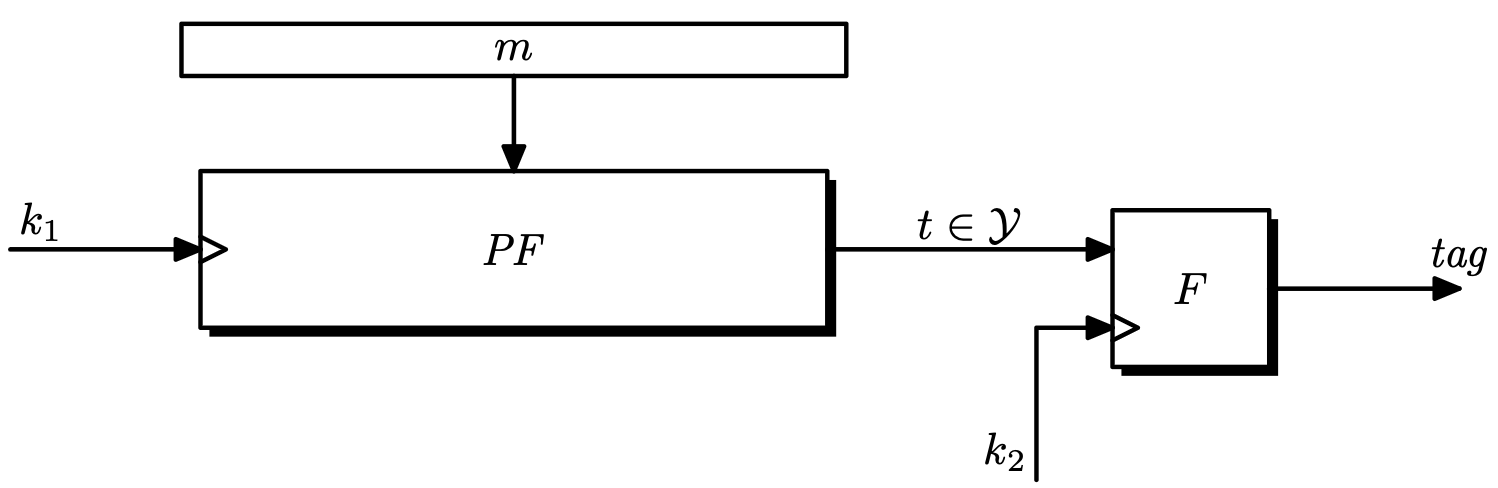
\includegraphics[width=0.65\linewidth]{figures/chapter6/fig4.png}
  \tikzset{every picture/.style={line width=0.75pt}} %set default line width to 0.75pt        

\begin{tikzpicture}[x=0.75pt,y=0.75pt,yscale=-1,xscale=1]
%uncomment if require: \path (0,160); %set diagram left start at 0, and has height of 160

%Shape: Rectangle [id:dp33326858691181327] 
\draw  [fill={rgb, 255:red, 255; green, 255; blue, 255 }  ,fill opacity=1 ][line width=1.2]  (50,0) -- (230,0) -- (230,20) -- (50,20) -- cycle ;
%Shape: Rectangle [id:dp083961736493265] 
\draw  [fill={rgb, 255:red, 255; green, 255; blue, 255 }  ,fill opacity=1 ][line width=1.2] [general shadow={fill=black,shadow xshift=2.25pt,shadow yshift=-2.25pt}] (300,60) -- (350,60) -- (350,110) -- (300,110) -- cycle ;
%Straight Lines [id:da7095405239206141] 
\draw    (350,85) -- (397,85) ;
\draw [shift={(400,85)}, rotate = 180] [fill={rgb, 255:red, 0; green, 0; blue, 0 }  ][line width=0.08]  [draw opacity=0] (7.14,-3.43) -- (0,0) -- (7.14,3.43) -- cycle    ;
%Straight Lines [id:da9545512828776872] 
\draw    (0,75) -- (47,75) ;
\draw [shift={(50,75)}, rotate = 180] [fill={rgb, 255:red, 0; green, 0; blue, 0 }  ][line width=0.08]  [draw opacity=0] (7.14,-3.43) -- (0,0) -- (7.14,3.43) -- cycle    ;
%Straight Lines [id:da15363507283754263] 
\draw    (140,20) -- (140,47) ;
\draw [shift={(140,50)}, rotate = 270] [fill={rgb, 255:red, 0; green, 0; blue, 0 }  ][line width=0.08]  [draw opacity=0] (7.14,-3.43) -- (0,0) -- (7.14,3.43) -- cycle    ;
%Straight Lines [id:da3074642964706582] 
\draw    (275,140) -- (275,95) -- (297,95) ;
\draw [shift={(300,95)}, rotate = 180] [fill={rgb, 255:red, 0; green, 0; blue, 0 }  ][line width=0.08]  [draw opacity=0] (7.14,-3.43) -- (0,0) -- (7.14,3.43) -- cycle    ;
%Flowchart: Extract [id:dp5425750567919283] 
\draw   (305,95) -- (300,98.5) -- (300,91.5) -- cycle ;
%Shape: Rectangle [id:dp7127919566797498] 
\draw  [fill={rgb, 255:red, 255; green, 255; blue, 255 }  ,fill opacity=1 ][line width=1.2] [general shadow={fill=black,shadow xshift=2.25pt,shadow yshift=-2.25pt}] (50,50) -- (230,50) -- (230,100) -- (50,100) -- cycle ;
%Flowchart: Extract [id:dp7415383977392733] 
\draw   (55,75) -- (50,78.5) -- (50,71.5) -- cycle ;
%Straight Lines [id:da7132747696931903] 
\draw    (230,75) -- (297,75) ;
\draw [shift={(300,75)}, rotate = 180] [fill={rgb, 255:red, 0; green, 0; blue, 0 }  ][line width=0.08]  [draw opacity=0] (7.14,-3.43) -- (0,0) -- (7.14,3.43) -- cycle    ;

% Text Node
\draw (325,85) node    {$F$};
% Text Node
\draw (140,10) node    {$m$};
% Text Node
\draw (400,81.6) node [anchor=south] [inner sep=0.75pt]    {$tag$};
% Text Node
\draw (2,71.6) node [anchor=south west] [inner sep=0.75pt]    {$k_{1}$};
% Text Node
\draw (140,75) node    {$PF$};
% Text Node
\draw (265,71.6) node [anchor=south] [inner sep=0.75pt]    {$t\in \mathcal{Y}$};
% Text Node
\draw (273,136.6) node [anchor=south east] [inner sep=0.75pt]    {$k_{2}$};


\end{tikzpicture}
  \caption{加密 PRF 构造 $EF(k,m)$}
  \label{fig:6-4}
\end{figure}

我们声称,当 $PF$ 是 CBC 或级联中的任何一种构造时,$EF$ 都是一个安全的 PRF。更一般地,我们表明,只要 $PF$ 是一个\emph{可扩展的} PRF,$EF$ 就是安全的。可扩展性的定义如下:

\begin{definition}\label{def:6-4}
令 $PF$ 是一个定义在 $(\mathcal{K},\mathcal{X}^{\leq\ell},\mathcal{Y})$ 上的 PRF。如果对于所有的 $k\in\mathcal{K}$,$x,y\in\mathcal{X}^{\leq\ell-1}$ 和 $a\in\mathcal{X}$,我们都有:
\[
\text{if}\quad
PF(k,x)=PF(k,y)
\quad\text{then}\quad
PF(k,\;x\,\Vert\,a)=PF(k,\;y\,\Vert\,a)
\]
就称 $PF$ 是一个\textbf{可扩展 (extendable) PRF}。
\end{definition}

不难发现,CBC 和级联构造都是可扩展的 PRF。下面的定理将表明,如果 $PF$ 是一个可扩展的无前缀安全 PRF,$EF$ 就是一个安全的 PRF。

\begin{theorem}\label{theo:6-5}
令 $PF$ 是一个定义在 $(\mathcal{K}_1,\mathcal{X}^{\leq\ell+1},\mathcal{Y})$ 上的可扩展且无前缀安全的 PRF,其中 $|\mathcal{Y}|$ 是超多项式的,$\ell$ 是多项式约束的。令 $F$ 是一个定义在 $(\mathcal{K}_2,\mathcal{Y},\mathcal{T})$ 上的安全的 PRF。那么如式 \ref{eq:6-17} 中所定义的 $EF$ 是一个定义在 $(\mathcal{K}_1\times\mathcal{K}_2,\mathcal{X}^{\leq\ell},\mathcal{T})$ 上的安全的 PRF。
\begin{quote}
特别地,对于每个按照攻击游戏 \ref{game:4-2} 攻击 $EF$ 的 PRF 对手 $\mathcal{A}$,假设它最多能够向其挑战者发起 $Q$ 次查询,则必然存在一个按照攻击游戏 \ref{game:4-2} 攻击 $F$ 的 PRF 对手 $\mathcal{B}_1$ 和一个按照攻击游戏 \ref{game:4-2} 攻击 $PF$ 的无前缀 PRF 对手 $\mathcal{B}_2$,其中 $\mathcal{B}_1$ 和 $\mathcal{B}_2$ 都是围绕 $\mathcal{A}$ 的基本包装器,满足:
\end{quote}
\begin{equation}\label{eq:6-18}
{\rm PRF\mathsf{adv}}[\mathcal{A},EF]\leq {\rm PRF\mathsf{adv}}[\mathcal{B}_1,F]+{\rm PRF^{pf}\mathsf{adv}}[\mathcal{B}_2,PF]+\frac{Q^2}{2|\mathcal{Y}|}
\end{equation}
\end{theorem}

\noindent
在我们提供了必要的工具之后,我们将在下一章(\ref{subsec:7-3-1} 小节)证明定理 \ref{theo:6-5}。请注意,为了使 $EF$ 在长度不超过 $\ell$ 的输入上都是安全的 PRF,该定理要求 $PF$ 对于长为 $\ell+1$ 的输入是都无前缀安全的。

\begin{snote}[式 \ref{eq:6-18} 中的上界是严格的。]
虽然不是完全必要,但让我们假设 $\mathcal{Y}=\mathcal{T}$,$F$ 是一个分组密码,并且 $|\mathcal{X}|$ 不是非常小。这些假设将大大简化论证。我们下面展示一种攻击,它能在 $Q\approx\sqrt{|\mathcal{Y}|}$ 次查询之后以恒定概率攻破 $EF$。事实上,我们的攻击将攻破作为一个 MAC 的 $EF$。对手首先挑选 $Q$ 个随机输入 $x_1,\dots,x_Q\in\mathcal{X}^2$,并用这 $Q$ 个输入向其挑战者发起查询,以得到应答 $t_1,\dots,t_Q\in\mathcal{T}$。根据生日悖论(推论 \ref{cor:B-2}),对于任何固定的密钥 $k_1$,存在不同的索引 $i$ 和 $j$ 使得 $x_i\neq x_j$ 且 $PF(k_1,x_i)=PF(k_1,x_j)$ 的概率是恒定的。一方面,如果发生这样的碰撞,我们可以有效发现它,这是因为对于这样的一对索引,必有 $t_i=t_j$。另一方面,如果存在一对索引 $i$ 和 $j$ 使得 $t_i=t_j$,由于我们假设 $F$ 是一个分组密码,那么必然有 $PF(k_1,x_i)=PF(k_1,x_j)$。现在,假设 $x_i\neq x_j$ 且 $PF(k_1,x_i)=PF(k_1,x_j)$,由于 $PF$ 是可扩展的,那么对于任意 $a\in\mathcal{X}$,我们都有 $PF\big(k_1,\,(x_i\,\Vert\,a)\big)=PF\big(k_1,\,(x_j\,\Vert\,a)\big)$。因此,我们的对手可以获得 $x_i\,\Vert\,a$ 的 MAC 标签 $t$,而这个标签 $t$ 同时也是 $x_j\,\Vert\,a$ 的有效标签。推广这一攻击,我们就能很容易地证明式 \ref{eq:6-18} 中 ${Q^2}/{(2|\mathcal{Y}|)}$ 这一项的必要性。
\end{snote}

\subsection{ECBC 和 NMAC:用于变长输入的安全 PRF}

图 \ref{fig:6-5-a} 和 \ref{fig:6-5-b} 展示了对 CBC 和级联应用 $EF$ 构造的结果。

\begin{figure}
  \centering
  \subfigure[ECBC 构造 $\mathrm{ECBC}(k,m)$(加密CBC)]{
    

\tikzset{every picture/.style={line width=0.75pt}} %set default line width to 0.75pt        

\begin{tikzpicture}[x=0.75pt,y=0.75pt,yscale=-1,xscale=1]
%uncomment if require: \path (0,181); %set diagram left start at 0, and has height of 181

%Shape: Rectangle [id:dp4443145165233573] 
\draw  [fill={rgb, 255:red, 255; green, 255; blue, 255 }  ,fill opacity=1 ][line width=1.2] [general shadow={fill=black,shadow xshift=2.25pt,shadow yshift=-2.25pt}] (10,90) -- (60,90) -- (60,140) -- (10,140) -- cycle ;
%Shape: Rectangle [id:dp3654823418270836] 
\draw  [fill={rgb, 255:red, 255; green, 255; blue, 255 }  ,fill opacity=1 ][line width=1.2] [general shadow={fill=black,shadow xshift=2.25pt,shadow yshift=-2.25pt}] (0,0) -- (70,0) -- (70,20) -- (0,20) -- cycle ;
%Shape: Rectangle [id:dp893088791780835] 
\draw  [fill={rgb, 255:red, 255; green, 255; blue, 255 }  ,fill opacity=1 ][line width=1.2] [general shadow={fill=black,shadow xshift=2.25pt,shadow yshift=-2.25pt}] (100,0) -- (170,0) -- (170,20) -- (100,20) -- cycle ;
%Shape: Rectangle [id:dp4783618167357453] 
\draw  [fill={rgb, 255:red, 255; green, 255; blue, 255 }  ,fill opacity=1 ][line width=1.2] [general shadow={fill=black,shadow xshift=2.25pt,shadow yshift=-2.25pt}] (200,0) -- (270,0) -- (270,20) -- (200,20) -- cycle ;
%Shape: Rectangle [id:dp14886948130262612] 
\draw  [fill={rgb, 255:red, 255; green, 255; blue, 255 }  ,fill opacity=1 ][line width=1.2] [general shadow={fill=black,shadow xshift=2.25pt,shadow yshift=-2.25pt}] (330,0) -- (400,0) -- (400,20) -- (330,20) -- cycle ;
%Shape: Rectangle [id:dp8119610043743812] 
\draw  [fill={rgb, 255:red, 255; green, 255; blue, 255 }  ,fill opacity=1 ][line width=1.2] [general shadow={fill=black,shadow xshift=2.25pt,shadow yshift=-2.25pt}] (110,90) -- (160,90) -- (160,140) -- (110,140) -- cycle ;
%Shape: Rectangle [id:dp18004760511222906] 
\draw  [fill={rgb, 255:red, 255; green, 255; blue, 255 }  ,fill opacity=1 ][line width=1.2] [general shadow={fill=black,shadow xshift=2.25pt,shadow yshift=-2.25pt}] (210,90) -- (260,90) -- (260,140) -- (210,140) -- cycle ;
%Shape: Rectangle [id:dp960423359685666] 
\draw  [fill={rgb, 255:red, 255; green, 255; blue, 255 }  ,fill opacity=1 ][line width=1.2] [general shadow={fill=black,shadow xshift=2.25pt,shadow yshift=-2.25pt}] (340,90) -- (390,90) -- (390,140) -- (340,140) -- cycle ;
%Straight Lines [id:da44373949352543574] 
\draw    (35,20) -- (35,87) ;
\draw [shift={(35,90)}, rotate = 270] [fill={rgb, 255:red, 0; green, 0; blue, 0 }  ][line width=0.08]  [draw opacity=0] (7.14,-3.43) -- (0,0) -- (7.14,3.43) -- cycle    ;
%Straight Lines [id:da38045035541987127] 
\draw    (60,115) -- (85,115) -- (85,55) -- (127,55) ;
\draw [shift={(130,55)}, rotate = 180] [fill={rgb, 255:red, 0; green, 0; blue, 0 }  ][line width=0.08]  [draw opacity=0] (7.14,-3.43) -- (0,0) -- (7.14,3.43) -- cycle    ;
%Straight Lines [id:da6694268861945114] 
\draw    (160,115) -- (185,115) -- (185,55) -- (227,55) ;
\draw [shift={(230,55)}, rotate = 180] [fill={rgb, 255:red, 0; green, 0; blue, 0 }  ][line width=0.08]  [draw opacity=0] (7.14,-3.43) -- (0,0) -- (7.14,3.43) -- cycle    ;
%Straight Lines [id:da1731188178152383] 
\draw    (330,55) -- (357,55) ;
\draw [shift={(360,55)}, rotate = 180] [fill={rgb, 255:red, 0; green, 0; blue, 0 }  ][line width=0.08]  [draw opacity=0] (7.14,-3.43) -- (0,0) -- (7.14,3.43) -- cycle    ;
%Straight Lines [id:da18974241223755217] 
\draw    (135,20) -- (135,47) ;
\draw [shift={(135,50)}, rotate = 270] [fill={rgb, 255:red, 0; green, 0; blue, 0 }  ][line width=0.08]  [draw opacity=0] (7.14,-3.43) -- (0,0) -- (7.14,3.43) -- cycle    ;
%Straight Lines [id:da9241213725477959] 
\draw    (135,60) -- (135,87) ;
\draw [shift={(135,90)}, rotate = 270] [fill={rgb, 255:red, 0; green, 0; blue, 0 }  ][line width=0.08]  [draw opacity=0] (7.14,-3.43) -- (0,0) -- (7.14,3.43) -- cycle    ;
%Straight Lines [id:da8064891185926979] 
\draw    (235,20) -- (235,47) ;
\draw [shift={(235,50)}, rotate = 270] [fill={rgb, 255:red, 0; green, 0; blue, 0 }  ][line width=0.08]  [draw opacity=0] (7.14,-3.43) -- (0,0) -- (7.14,3.43) -- cycle    ;
%Straight Lines [id:da20365370380672698] 
\draw    (365,20) -- (365,47) ;
\draw [shift={(365,50)}, rotate = 270] [fill={rgb, 255:red, 0; green, 0; blue, 0 }  ][line width=0.08]  [draw opacity=0] (7.14,-3.43) -- (0,0) -- (7.14,3.43) -- cycle    ;
%Straight Lines [id:da8209148833770106] 
\draw    (235,60) -- (235,87) ;
\draw [shift={(235,90)}, rotate = 270] [fill={rgb, 255:red, 0; green, 0; blue, 0 }  ][line width=0.08]  [draw opacity=0] (7.14,-3.43) -- (0,0) -- (7.14,3.43) -- cycle    ;
%Straight Lines [id:da41897506139568685] 
\draw    (365,60) -- (365,87) ;
\draw [shift={(365,90)}, rotate = 270] [fill={rgb, 255:red, 0; green, 0; blue, 0 }  ][line width=0.08]  [draw opacity=0] (7.14,-3.43) -- (0,0) -- (7.14,3.43) -- cycle    ;
%Straight Lines [id:da5786817284582193] 
\draw    (260,115) -- (285,115) ;
%Straight Lines [id:da354850726992592] 
\draw  [dash pattern={on 0.84pt off 2.51pt}]  (285,115) -- (310,115) -- (310,55) -- (330,55) ;
%Straight Lines [id:da7935744551156634] 
\draw    (490,115) -- (537,115) ;
\draw [shift={(540,115)}, rotate = 180] [fill={rgb, 255:red, 0; green, 0; blue, 0 }  ][line width=0.08]  [draw opacity=0] (7.14,-3.43) -- (0,0) -- (7.14,3.43) -- cycle    ;
%Shape: Rectangle [id:dp5498562140150316] 
\draw  [fill={rgb, 255:red, 255; green, 255; blue, 255 }  ,fill opacity=1 ][line width=1.2] [general shadow={fill=black,shadow xshift=2.25pt,shadow yshift=-2.25pt}] (440,90) -- (490,90) -- (490,140) -- (440,140) -- cycle ;
%Straight Lines [id:da297515876064387] 
\draw    (390,115) -- (437,115) ;
\draw [shift={(440,115)}, rotate = 180] [fill={rgb, 255:red, 0; green, 0; blue, 0 }  ][line width=0.08]  [draw opacity=0] (7.14,-3.43) -- (0,0) -- (7.14,3.43) -- cycle    ;
%Straight Lines [id:da29951358036034725] 
\draw  [dash pattern={on 4.5pt off 4.5pt}]  (0,165) -- (400,165) ;
\draw [shift={(400,165)}, rotate = 180] [color={rgb, 255:red, 0; green, 0; blue, 0 }  ][line width=0.75]    (0,4.47) -- (0,-4.47)   ;
\draw [shift={(0,165)}, rotate = 180] [color={rgb, 255:red, 0; green, 0; blue, 0 }  ][line width=0.75]    (0,4.47) -- (0,-4.47)   ;
%Shape: Rectangle [id:dp3234507369689261] 
\draw  [draw opacity=0][fill={rgb, 255:red, 255; green, 255; blue, 255 }  ,fill opacity=1 ] (175,155) -- (225,155) -- (225,175) -- (175,175) -- cycle ;

% Text Node
\draw (35,115) node    {$F( k_{1} ,\cdot )$};
% Text Node
\draw (135,115) node    {$F( k_{1} ,\cdot )$};
% Text Node
\draw (235,115) node    {$F( k_{1} ,\cdot )$};
% Text Node
\draw (365,115) node    {$F( k_{1} ,\cdot )$};
% Text Node
\draw (135,55) node  [font=\large]  {$\oplus $};
% Text Node
\draw (235,55) node  [font=\large]  {$\oplus $};
% Text Node
\draw (365,55) node  [font=\large]  {$\oplus $};
% Text Node
\draw (300,10) node    {$\cdots $};
% Text Node
\draw (35,10) node    {$a_{1}$};
% Text Node
\draw (135,10) node    {$a_{2}$};
% Text Node
\draw (235,10) node    {$a_{3}$};
% Text Node
\draw (365,10) node    {$a_{\ell }$};
% Text Node
\draw (540,111.6) node [anchor=south] [inner sep=0.75pt]    {$tag$};
% Text Node
\draw (465,115) node    {$F( k_{2} ,\cdot )$};
% Text Node
\draw (200,165) node   [align=left] {CBC};


\end{tikzpicture}
  	\label{fig:6-5-a}
  }
  
  \,
  
  \,
  
  \subfigure[NMAC 构造 $\mathrm{NMAC}(k,m)$(加密级联)]{
  	

\tikzset{every picture/.style={line width=0.75pt}} %set default line width to 0.75pt        

\begin{tikzpicture}[x=0.75pt,y=0.75pt,yscale=-1,xscale=1]
%uncomment if require: \path (0,182); %set diagram left start at 0, and has height of 182

%Shape: Rectangle [id:dp8247531494470199] 
\draw  [fill={rgb, 255:red, 255; green, 255; blue, 255 }  ,fill opacity=1 ][line width=1.2] [general shadow={fill=black,shadow xshift=2.25pt,shadow yshift=-2.25pt}] (50,50) -- (100,50) -- (100,100) -- (50,100) -- cycle ;
%Shape: Rectangle [id:dp6129441991681601] 
\draw  [fill={rgb, 255:red, 255; green, 255; blue, 255 }  ,fill opacity=1 ][line width=1.2] [general shadow={fill=black,shadow xshift=2.25pt,shadow yshift=-2.25pt}] (40,0) -- (110,0) -- (110,20) -- (40,20) -- cycle ;
%Shape: Rectangle [id:dp90829523247659] 
\draw  [fill={rgb, 255:red, 255; green, 255; blue, 255 }  ,fill opacity=1 ][line width=1.2] [general shadow={fill=black,shadow xshift=2.25pt,shadow yshift=-2.25pt}] (140,0) -- (210,0) -- (210,20) -- (140,20) -- cycle ;
%Shape: Rectangle [id:dp08202625686221188] 
\draw  [fill={rgb, 255:red, 255; green, 255; blue, 255 }  ,fill opacity=1 ][line width=1.2] [general shadow={fill=black,shadow xshift=2.25pt,shadow yshift=-2.25pt}] (270,0) -- (340,0) -- (340,20) -- (270,20) -- cycle ;
%Shape: Rectangle [id:dp9192770861603901] 
\draw  [fill={rgb, 255:red, 255; green, 255; blue, 255 }  ,fill opacity=1 ][line width=1.2] [general shadow={fill=black,shadow xshift=2.25pt,shadow yshift=-2.25pt}] (150,50) -- (200,50) -- (200,100) -- (150,100) -- cycle ;
%Shape: Rectangle [id:dp6226214384270212] 
\draw  [fill={rgb, 255:red, 255; green, 255; blue, 255 }  ,fill opacity=1 ][line width=1.2] [general shadow={fill=black,shadow xshift=2.25pt,shadow yshift=-2.25pt}] (280,50) -- (330,50) -- (330,100) -- (280,100) -- cycle ;
%Straight Lines [id:da593286075335618] 
\draw    (100,75) -- (147,75) ;
\draw [shift={(150,75)}, rotate = 180] [fill={rgb, 255:red, 0; green, 0; blue, 0 }  ][line width=0.08]  [draw opacity=0] (7.14,-3.43) -- (0,0) -- (7.14,3.43) -- cycle    ;
%Straight Lines [id:da362450281296391] 
\draw    (175,20) -- (175,47) ;
\draw [shift={(175,50)}, rotate = 270] [fill={rgb, 255:red, 0; green, 0; blue, 0 }  ][line width=0.08]  [draw opacity=0] (7.14,-3.43) -- (0,0) -- (7.14,3.43) -- cycle    ;
%Straight Lines [id:da04154463636417449] 
\draw    (305,20) -- (305,47) ;
\draw [shift={(305,50)}, rotate = 270] [fill={rgb, 255:red, 0; green, 0; blue, 0 }  ][line width=0.08]  [draw opacity=0] (7.14,-3.43) -- (0,0) -- (7.14,3.43) -- cycle    ;
%Straight Lines [id:da932866823555605] 
\draw    (330,75) -- (397,75) ;
\draw [shift={(400,75)}, rotate = 180] [fill={rgb, 255:red, 0; green, 0; blue, 0 }  ][line width=0.08]  [draw opacity=0] (7.14,-3.43) -- (0,0) -- (7.14,3.43) -- cycle    ;
%Straight Lines [id:da5223337867158735] 
\draw    (0,75) -- (47,75) ;
\draw [shift={(50,75)}, rotate = 180] [fill={rgb, 255:red, 0; green, 0; blue, 0 }  ][line width=0.08]  [draw opacity=0] (7.14,-3.43) -- (0,0) -- (7.14,3.43) -- cycle    ;
%Straight Lines [id:da7098873699377382] 
\draw    (75,20) -- (75,47) ;
\draw [shift={(75,50)}, rotate = 270] [fill={rgb, 255:red, 0; green, 0; blue, 0 }  ][line width=0.08]  [draw opacity=0] (7.14,-3.43) -- (0,0) -- (7.14,3.43) -- cycle    ;
%Straight Lines [id:da439501690083433] 
\draw    (255,75) -- (277,75) ;
\draw [shift={(280,75)}, rotate = 180] [fill={rgb, 255:red, 0; green, 0; blue, 0 }  ][line width=0.08]  [draw opacity=0] (7.14,-3.43) -- (0,0) -- (7.14,3.43) -- cycle    ;
%Flowchart: Extract [id:dp7891990374519424] 
\draw   (55,75) -- (50,78.5) -- (50,71.5) -- cycle ;
%Flowchart: Extract [id:dp34101688013357156] 
\draw   (155,75) -- (150,78.5) -- (150,71.5) -- cycle ;
%Flowchart: Extract [id:dp09601501443221516] 
\draw   (285,75) -- (280,78.5) -- (280,71.5) -- cycle ;
%Straight Lines [id:da6114907985079976] 
\draw    (200,75) -- (225,75) ;
%Straight Lines [id:da7083024016134647] 
\draw  [dash pattern={on 0.84pt off 2.51pt}]  (225,75) -- (255,75) ;
%Shape: Rectangle [id:dp10815488481380497] 
\draw  [fill={rgb, 255:red, 255; green, 255; blue, 255 }  ,fill opacity=1 ][line width=1.2]  (400,65) -- (470,65) -- (470,85) -- (400,85) -- cycle ;
%Shape: Rectangle [id:dp22568098998466568] 
\draw  [fill={rgb, 255:red, 255; green, 255; blue, 255 }  ,fill opacity=1 ][line width=1.2] [general shadow={fill=black,shadow xshift=2.25pt,shadow yshift=-2.25pt}] (410,115) -- (460,115) -- (460,165) -- (410,165) -- cycle ;
%Straight Lines [id:da00862867995476968] 
\draw    (435,85) -- (435,112) ;
\draw [shift={(435,115)}, rotate = 270] [fill={rgb, 255:red, 0; green, 0; blue, 0 }  ][line width=0.08]  [draw opacity=0] (7.14,-3.43) -- (0,0) -- (7.14,3.43) -- cycle    ;
%Flowchart: Extract [id:dp9906642278151132] 
\draw   (415,140) -- (410,143.5) -- (410,136.5) -- cycle ;
%Straight Lines [id:da13089111893227923] 
\draw    (460,140) -- (507,140) ;
\draw [shift={(510,140)}, rotate = 180] [fill={rgb, 255:red, 0; green, 0; blue, 0 }  ][line width=0.08]  [draw opacity=0] (7.14,-3.43) -- (0,0) -- (7.14,3.43) -- cycle    ;
%Straight Lines [id:da8153858801598555] 
\draw    (380,140) -- (407,140) ;
\draw [shift={(410,140)}, rotate = 180] [fill={rgb, 255:red, 0; green, 0; blue, 0 }  ][line width=0.08]  [draw opacity=0] (7.14,-3.43) -- (0,0) -- (7.14,3.43) -- cycle    ;
%Straight Lines [id:da8236950032942283] 
\draw  [dash pattern={on 4.5pt off 4.5pt}]  (40,125) -- (340,125) ;
\draw [shift={(340,125)}, rotate = 180] [color={rgb, 255:red, 0; green, 0; blue, 0 }  ][line width=0.75]    (0,4.47) -- (0,-4.47)   ;
\draw [shift={(40,125)}, rotate = 180] [color={rgb, 255:red, 0; green, 0; blue, 0 }  ][line width=0.75]    (0,4.47) -- (0,-4.47)   ;
%Shape: Rectangle [id:dp8129886574905969] 
\draw  [draw opacity=0][fill={rgb, 255:red, 255; green, 255; blue, 255 }  ,fill opacity=1 ] (160,115) -- (220,115) -- (220,135) -- (160,135) -- cycle;

% Text Node
\draw (75,75) node    {$F$};
% Text Node
\draw (175,75) node    {$F$};
% Text Node
\draw (305,75) node    {$F$};
% Text Node
\draw (240,10) node    {$\cdots $};
% Text Node
\draw (75,10) node    {$a_{1}$};
% Text Node
\draw (175,10) node    {$a_{2}$};
% Text Node
\draw (305,10) node    {$a_{\ell }$};
% Text Node
\draw (510,136.6) node [anchor=south] [inner sep=0.75pt]    {$tag$};
% Text Node
\draw (2,71.6) node [anchor=south west] [inner sep=0.75pt]    {$k_{1}$};
% Text Node
\draw (435,75) node    {$t\;\|\;\mathsf{fpad}$};
% Text Node
\draw (435,140) node    {$F$};
% Text Node
\draw (365,71.6) node [anchor=south] [inner sep=0.75pt]    {$t\in \mathcal{K}$};
% Text Node
\draw (378,140) node [anchor=east] [inner sep=0.75pt]    {$k_{2}$};
% Text Node
\draw (190,125) node   [align=left] {级联};


\end{tikzpicture}
  	\label{fig:6-5-b}
  }
  \caption{用于变长输入的安全 PRF}
\end{figure}

\subsubsection{加密 CBC PRF}

将 $EF$ 应用于 CBC 构造就能得到一个经典的 PRF(因而也是一个 MAC),称为\textbf{加密 CBC (encrypted-CBC)} 或 \textbf{ECBC}。这种 MAC 由 ANSI 标准化(见 \ref{sec:6-9} 节),并被广泛用于银行业。ECBC PRF 在 CBC 和最终的加密中使用相同的底层 PRF $F$。因此,ECBC 定义在 $(\mathcal{K}^2,\mathcal{X}^{\leq\ell+1},\mathcal{X})$ 上。

\begin{theorem}[ECBC 的安全性]\label{theo:6-6}
令 $F$ 是一个定义在 $(\mathcal{K},\mathcal{X},\mathcal{X})$ 上的安全 PRF。假设 $\mathcal{X}$ 是超多项式的,$\ell$ 是一个多项式约束的长度参数。那么 ECBC 是一个定义在 $(\mathcal{K}^2,\mathcal{X}^{\leq\ell+1},\mathcal{X})$ 上的安全 PRF。
\begin{quote}
特别地,对于每个按照攻击游戏 \ref{game:4-2} 攻击 ECBC 的 PRF 对手 $\mathcal{A}$,假设它最多能够向其挑战者发起 $Q$ 次查询,则必然存在两个按照攻击游戏 \ref{game:4-2} 攻击 $F$ 的 PRF 对手 $\mathcal{B}_1$ 和 $\mathcal{B}_2$,其中 $\mathcal{B}_1$ 和 $\mathcal{B}_2$ 都是围绕 $\mathcal{A}$ 的基本包装器,满足:
\end{quote}
\begin{equation}\label{eq:6-19}
{\rm PRF}\mathsf{adv}[\mathcal{A},{\rm ECBC}]\leq{\rm PRF}\mathsf{adv}[\mathcal{B}_1,F]+{\rm PRF}\mathsf{adv}[\mathcal{B}_2,F]+\frac{(Q(l+1))^2+Q^2}{2|\mathcal{X}|}
\end{equation}
\end{theorem}

\begin{proof}
根据定理 \ref{theo:6-3},CBC 显然是可扩展的,而且是一个无前缀安全的 PRF。因此,如果底层 PRF $F$ 是安全的,那么根据定理 \ref{theo:6-5},ECBC 也是一个安全的 PRF。
\end{proof}

定理 \ref{theo:6-5} 之后的论证表明,存在一个攻击者,在 $Q\approx\sqrt{|\mathcal{X}|}$ 次查询后,能以恒定优势破解该 PRF。回顾一下,对于 3DES,我们有 $\mathcal{X}=\{0,1\}^{64}$。因此,在大约 10 亿次(或者更准确地说, $2^{32}$ 次)查询之后,攻击者就能以恒定的概率破解 ECBC-3DES MAC。

\subsubsection{NMAC PRF}

将 $EF$ 应用于级联构造同样能得到一个 PRF(因而也是一个 MAC),称为\textbf{嵌套 MAC (Nested MAC)} 或 \textbf{NMAC}。这种 MAC 的一个变体由 IETF 标准化(见 \ref{subsec:8-7-2} 小节),并被广泛用于互联网协议中。

我们希望使用相同的底层 PRF $F$ 来构造级联和进行最终的加密。但不幸的是,级联的输出在 $\mathcal{K}$ 上,而 $F$ 的输入在 $\mathcal{X}$ 上。为了解决这个问题,我们需要将级联的输出嵌入到 $\mathcal{X}$ 中。更确切地说,我们假设 $|\mathcal{K}|\leq|\mathcal{X}|$,并且有一个可有效计算的双射 $g$,它能将 $\mathcal{K}$ 中的元素映射到 $\mathcal{X}$ 上。比如说,假设 $\mathcal{K}:=\{0,1\}^\kappa$,$\mathcal{X}:=\{0,1\}^n$,其中 $\kappa\leq n$。我们定义 $g(t):=t\,\Vert\,\mathsf{fpad}$,其中 $\mathsf{fpad}$ 是一串 $n-\kappa$ 比特的固定填充序列。这个 $\mathsf{fpad}$ 可以像一串 $0$ 一样简单。通过这种转换,所有的 NMAC 都可以由一个安全的 PRF $F$ 构造出来,就如图 \ref{fig:6-5-b} 所示。

\begin{theorem}[NMAC 的安全性]\label{theo:6-7}
令 $F$ 是一个定义在 $(\mathcal{K},\mathcal{X},\mathcal{K})$ 上的安全的 PRF,其中 $\mathcal{K}$ 可以嵌入到 $\mathcal{X}$ 中,那么 NMAC 就是一个定义在 $(\mathcal{K}^2,\mathcal{X}^{\leq\ell},\mathcal{K})$ 上的安全的 PRF。
\begin{quote}
特别地,对于每个按照攻击游戏 \ref{game:4-2} 攻击 NMAC 的 PRF 对手 $\mathcal{A}$,假设它最多能够向其挑战者发起 $Q$ 次查询,则必然存在两个按照攻击游戏 \ref{game:4-2} 攻击 $F$ 的 PRF 对手 $\mathcal{B}_1$ 和 $\mathcal{B}_2$,其中 $\mathcal{B}_1$ 和 $\mathcal{B}_2$ 都是围绕 $\mathcal{A}$ 的基本包装器,满足:
\end{quote}
\begin{equation}\label{eq:6-20}
{\rm PRF}\mathsf{adv}[\mathcal{A},{\rm NMAC}]\leq (Q(\ell+1))\cdot{\rm PRF}\mathsf{adv}[\mathcal{B}_1,F]+{\rm PRF}\mathsf{adv}[\mathcal{B}_2,F]+\frac{Q^2}{2|\mathcal{K}|}
\end{equation}
\end{theorem}

\begin{proof}
根据定理 \ref{theo:6-4},NMAC 显然是可扩展的,而且是一个无前缀安全的 PRF。因此,如果底层 PRF $F$ 是安全的,那么根据定理 \ref{theo:6-5},NMAC 也是一个安全的 PRF。
\end{proof}

\begin{snote}[ECBC 和 NMAC 都是流式 MAC。]
ECBC 和 NMAC 都可以用来认证 $\mathcal{X}^{\leq l}$ 上的变长消息。此外,我们并不需要提前知晓消息的长度。具有这种特性的 MAC 被称为\textbf{流式 MAC (streaming MAC)}。这一特性使得应用程序能够一次向 MAC 提供一个消息分组,并在任意位置决定消息是否结束。这对于像流媒体视频这样的应用很重要,因为在这种应用中,应用程序也无法预知消息的长度。

相比之下,一些 MAC 系统要求将消息长度预加到消息正文中(见 \ref{sec:6-6} 节)。这样的 MAC 在实践中更难使用,因为它们要求应用程序在开始计算 MAC 之前就确定消息的长度。
\end{snote}
\section{从无前缀安全 PRF 到完全安全 PRF(方法 2):无前缀编码}\label{sec:6-6}

将无前缀安全的 PRF 转换为安全 PRF 的另一种方法是对 PRF 的输入进行编码,使得没有任何一条编码后的输入是另一条的前缀。我们定义以下术语:
\begin{itemize}
	\item 如果 $S\subseteq\mathcal{X}^{\leq\ell}$ 中的任何元素都不是其他元素的前缀,我们就称 $S$ 是一个\textbf{无前缀集 (prefix-free set)}。例如,如果 $(x_1,x_2,x_3)$ 属于一个无前缀集 $S$,那么 $x_1$ 和 $(x_1,x_2)$ 都不在 $S$ 中。
	\item 令 $\mathcal{X}^{\leq\ell}_{_{>0}}$ 表示$\mathcal{X}$ 上所有长度不超过 $\ell$ 的非空序列的集合。如果映射 $pf$ 是一个单射(即一对一函数),且 $pf$ 的像是一个无前缀集,我们就称 $pf:\mathcal{M}\to\mathcal{X}^{\leq\ell}_{_{>0}}$ 是一个\textbf{无前缀编码 (prefix-free encoding)}。
\end{itemize}

令 $PF$ 是一个定义在 $(\mathcal{K},\mathcal{X}^{\leq\ell},\mathcal{Y})$ 上的无前缀安全 PRF,且 $pf:\mathcal{M}\to\mathcal{X}^{\leq\ell}_{_{>0}}$ 是一个无前缀编码。定义派生的 PRF $F$ 为:
\[
F(k,m):=PF(k,pf(m))
\]
那么 $F$ 定义在 $(\mathcal{K},\mathcal{M},\mathcal{Y})$ 上。于是,我们就可以得到下面的定理。

\begin{theorem}\label{theo:6-8}
如果 $PF$ 是一个无前缀安全的 PRF,$pf$ 是一个无前缀编码,那么 $F$ 是一个安全的 PRF。
\end{theorem}

\subsection{无前缀编码}\label{subsec:6-6-1}

为了使用定理 \ref{theo:6-8} 构造 PRF,我们介绍两种无前缀编码 $pf:\mathcal{M}\to\mathcal{X}^{\leq\ell}$。我们假设 $\mathcal{X}=\{0,1\}^n$,其中 $n$ 是某个整数。

\begin{snote}[方法 1:前置长度。]
设 $\mathcal{M}:=\mathcal{X}^{\leq\ell-1}$,并令 $m=(a_1,\dots,a_v)\in\mathcal{M}$。定义:
\[
pf(m):=(\langle v\rangle,a_1,\dots,a_v)\quad\in\mathcal{X}^{\leq\ell}_{_{>0}}
\]
其中 $\langle v\rangle\in\mathcal{X}$ 是 $v$ 的二进制表示,即 $m$ 的长度。我们假设 $\ell<2^n$,那么消息长度可以被编码为 $n$ 比特的二进制序列。

我们下面论证 $pf$ 是一个无前缀编码。首先,$pf$ 显然是一个单射。为了说明 $pf$ 的像是一个无前缀集,令 $pf(x)$ 和 $pf(y)$ 是 $pf$ 的像中的两个元素。如果 $pf(x)$ 和 $pf(y)$ 包含相同数量的分组,那么它们中的任何一个都不可能是另一个的真前缀。如果 $pf(x)$ 和 $pf(y)$ 包含不同数量的分组,它们就必须在第一个分组上就有所不同,此时它们也同样都不可能是另一个的真前缀。因此,$pf$ 是一个无前缀编码。

这种无前缀编码在实践中并不常用,因为这样所产生的 MAC 不是一个流式 MAC:使用这种 MAC 的应用程序必须提前把消息的长度承诺给 MAC。正如我们之前所说,这对于流媒体应用来说极不实用,因为在这种应用中,数据包的长度可能无法提前预知。
\end{snote}

\begin{snote}[方法 2:停止比特。]
设 $\mathcal{\bar{X}}:=\{0,1\}^{n-1}$,并令 $\mathcal{M}=\mathcal{\bar{X}}^{\leq\ell}_{_{>0}}$。对于 $m=(a_1,\dots,a_v)\in\mathcal{M}$,定义:
\[
pf(m):=\big((a_1\,\Vert\,0),\,(a_2\,\Vert\,0),\,\dots,\,(a_{v-1}\,\Vert\,0),\,(a_v\,\Vert\,1)\big)\quad\in\mathcal{X}^{\leq\ell}_{_{>0}}
\]
显然,$pf$ 是一个单射。为了说明 $pf$ 的像是一个无前缀集,令 $pf(x)$ 和 $pf(y)$ 是 $pf$ 的像中的两个元素。设 $v$ 是 $pf(x)$ 中分组的数量。如果 $pf(y)$ 包含 $v$ 个或更少的分组,那么 $pf(x)$ 必然不是 $pf(y)$ 的真前缀。如果 $pf(y)$ 包含多于 $v$ 个分组,那么 $pf(y)$ 中的 $v$ 号分组以 $0$ 结束,而 $pf(x)$ 中的 $v$ 号分组以 $1$ 结束。因此,$pf(x)$ 和 $pf(y)$ 在 $v$ 号分组上有所不同,所以 $pf(x)$ 不是 $pf(y)$ 的真前缀。

这种无前缀编码所产生的 MAC 是一个流式 MAC。然而,这种编码使 MAC 的长度增加了 $v$ 比特。当使用 CBC 或级联计算一个长消息的 MAC 时,这种编码将导致对底层 PRF(比如 AES)的额外计算。相对地,\ref{sec:6-5} 节中介绍的加密 PRF 方法只增加了一次对底层 PRF 的计算。例如,使用 ECBC-AES 和 $pf$ 对一兆字节 ($2^{20}$ 字节) 的消息计算 MAC,除了加密 PRF 方法所需要的,还需要对 AES 进行额外的 $511$ 次评估。在实践中,情况甚至可能更糟。由于计算机更喜欢字节对齐的数据,我们很可能需要在每个分组中附加一整个字节,而不是仅仅一个比特。那么,使用 ECBC-AES 和 $pf$ 对一兆字节的消息计算 MAC,将导致比加密 PRF 方法多出 $4096$ 次 AES 的计算,大约多 $6\%$ 的开销。
\end{snote}
\section{从无前缀安全PRF到完全安全PRF(方法3):CMAC}\label{sec:6-7}

上一节中介绍的两种无前缀编码方法都有问题。第一种方法产生的 MAC 是非流式的,而第二种方法对于长的消息需要对底层的 PRF 进行更多的计算。我们可以将无前缀编码进行随机化处理来进一步地改进设计。我们下面建立一个流式且安全的 PRF,除了底层的无前缀安全 PRF 之外,该设计不会引入任何额外的开销。图 \ref{fig:6-6} 展示了这样的 MAC,它比从加密 PRF 或者确定性编码得到的 MAC 都要优秀。这种方法被用于 NIST 的一种 MAC 标准,称为 CMAC,我们将在 \ref{sec:6-10} 节中介绍它。

\begin{figure}
  \centering
  \subfigure[应用于 CBC 的 $rpf$]{
    

\tikzset{every picture/.style={line width=0.75pt}} %set default line width to 0.75pt        

\begin{tikzpicture}[x=0.75pt,y=0.75pt,yscale=-1,xscale=1]
%uncomment if require: \path (0,158); %set diagram left start at 0, and has height of 158

%Shape: Rectangle [id:dp4182993422972734] 
\draw  [fill={rgb, 255:red, 255; green, 255; blue, 255 }  ,fill opacity=1 ][line width=1.2] [general shadow={fill=black,shadow xshift=2.25pt,shadow yshift=-2.25pt}] (10,90) -- (60,90) -- (60,140) -- (10,140) -- cycle ;
%Shape: Rectangle [id:dp13722175757533117] 
\draw  [fill={rgb, 255:red, 255; green, 255; blue, 255 }  ,fill opacity=1 ][line width=1.2] [general shadow={fill=black,shadow xshift=2.25pt,shadow yshift=-2.25pt}] (0,0) -- (70,0) -- (70,20) -- (0,20) -- cycle ;
%Shape: Rectangle [id:dp6079517396133325] 
\draw  [fill={rgb, 255:red, 255; green, 255; blue, 255 }  ,fill opacity=1 ][line width=1.2] [general shadow={fill=black,shadow xshift=2.25pt,shadow yshift=-2.25pt}] (100,0) -- (170,0) -- (170,20) -- (100,20) -- cycle ;
%Shape: Rectangle [id:dp9852794728819017] 
\draw  [fill={rgb, 255:red, 255; green, 255; blue, 255 }  ,fill opacity=1 ][line width=1.2] [general shadow={fill=black,shadow xshift=2.25pt,shadow yshift=-2.25pt}] (200,0) -- (270,0) -- (270,20) -- (200,20) -- cycle ;
%Shape: Rectangle [id:dp6116986251464251] 
\draw  [fill={rgb, 255:red, 255; green, 255; blue, 255 }  ,fill opacity=1 ][line width=1.2] [general shadow={fill=black,shadow xshift=2.25pt,shadow yshift=-2.25pt}] (330,0) -- (400,0) -- (400,20) -- (330,20) -- cycle ;
%Shape: Rectangle [id:dp10666113902168184] 
\draw  [fill={rgb, 255:red, 255; green, 255; blue, 255 }  ,fill opacity=1 ][line width=1.2] [general shadow={fill=black,shadow xshift=2.25pt,shadow yshift=-2.25pt}] (110,90) -- (160,90) -- (160,140) -- (110,140) -- cycle ;
%Shape: Rectangle [id:dp34056482509437047] 
\draw  [fill={rgb, 255:red, 255; green, 255; blue, 255 }  ,fill opacity=1 ][line width=1.2] [general shadow={fill=black,shadow xshift=2.25pt,shadow yshift=-2.25pt}] (210,90) -- (260,90) -- (260,140) -- (210,140) -- cycle ;
%Shape: Rectangle [id:dp8689195597849015] 
\draw  [fill={rgb, 255:red, 255; green, 255; blue, 255 }  ,fill opacity=1 ][line width=1.2] [general shadow={fill=black,shadow xshift=2.25pt,shadow yshift=-2.25pt}] (340,90) -- (390,90) -- (390,140) -- (340,140) -- cycle ;
%Straight Lines [id:da5990381315424871] 
\draw    (35,20) -- (35,87) ;
\draw [shift={(35,90)}, rotate = 270] [fill={rgb, 255:red, 0; green, 0; blue, 0 }  ][line width=0.08]  [draw opacity=0] (7.14,-3.43) -- (0,0) -- (7.14,3.43) -- cycle    ;
%Straight Lines [id:da8398719505256165] 
\draw    (60,115) -- (85,115) -- (85,55) -- (127,55) ;
\draw [shift={(130,55)}, rotate = 180] [fill={rgb, 255:red, 0; green, 0; blue, 0 }  ][line width=0.08]  [draw opacity=0] (7.14,-3.43) -- (0,0) -- (7.14,3.43) -- cycle    ;
%Straight Lines [id:da0009868508709764967] 
\draw    (160,115) -- (185,115) -- (185,55) -- (227,55) ;
\draw [shift={(230,55)}, rotate = 180] [fill={rgb, 255:red, 0; green, 0; blue, 0 }  ][line width=0.08]  [draw opacity=0] (7.14,-3.43) -- (0,0) -- (7.14,3.43) -- cycle    ;
%Straight Lines [id:da025473096299675424] 
\draw    (330,55) -- (357,55) ;
\draw [shift={(360,55)}, rotate = 180] [fill={rgb, 255:red, 0; green, 0; blue, 0 }  ][line width=0.08]  [draw opacity=0] (7.14,-3.43) -- (0,0) -- (7.14,3.43) -- cycle    ;
%Straight Lines [id:da31427053673861094] 
\draw    (135,20) -- (135,47) ;
\draw [shift={(135,50)}, rotate = 270] [fill={rgb, 255:red, 0; green, 0; blue, 0 }  ][line width=0.08]  [draw opacity=0] (7.14,-3.43) -- (0,0) -- (7.14,3.43) -- cycle    ;
%Straight Lines [id:da003713886257406651] 
\draw    (135,60) -- (135,87) ;
\draw [shift={(135,90)}, rotate = 270] [fill={rgb, 255:red, 0; green, 0; blue, 0 }  ][line width=0.08]  [draw opacity=0] (7.14,-3.43) -- (0,0) -- (7.14,3.43) -- cycle    ;
%Straight Lines [id:da48425819515088664] 
\draw    (235,20) -- (235,47) ;
\draw [shift={(235,50)}, rotate = 270] [fill={rgb, 255:red, 0; green, 0; blue, 0 }  ][line width=0.08]  [draw opacity=0] (7.14,-3.43) -- (0,0) -- (7.14,3.43) -- cycle    ;
%Straight Lines [id:da0745686777480592] 
\draw    (365,20) -- (365,47) ;
\draw [shift={(365,50)}, rotate = 270] [fill={rgb, 255:red, 0; green, 0; blue, 0 }  ][line width=0.08]  [draw opacity=0] (7.14,-3.43) -- (0,0) -- (7.14,3.43) -- cycle    ;
%Straight Lines [id:da522297969720648] 
\draw    (235,60) -- (235,87) ;
\draw [shift={(235,90)}, rotate = 270] [fill={rgb, 255:red, 0; green, 0; blue, 0 }  ][line width=0.08]  [draw opacity=0] (7.14,-3.43) -- (0,0) -- (7.14,3.43) -- cycle    ;
%Straight Lines [id:da7275998801342789] 
\draw    (365,60) -- (365,87) ;
\draw [shift={(365,90)}, rotate = 270] [fill={rgb, 255:red, 0; green, 0; blue, 0 }  ][line width=0.08]  [draw opacity=0] (7.14,-3.43) -- (0,0) -- (7.14,3.43) -- cycle    ;
%Straight Lines [id:da5036470587832664] 
\draw    (260,115) -- (285,115) ;
%Straight Lines [id:da5900182340547888] 
\draw  [dash pattern={on 0.84pt off 2.51pt}]  (285,115) -- (310,115) -- (310,55) -- (330,55) ;
%Straight Lines [id:da35743013601482265] 
\draw    (390,115) -- (437,115) ;
\draw [shift={(440,115)}, rotate = 180] [fill={rgb, 255:red, 0; green, 0; blue, 0 }  ][line width=0.08]  [draw opacity=0] (7.14,-3.43) -- (0,0) -- (7.14,3.43) -- cycle    ;
%Straight Lines [id:da29748517743722713] 
\draw    (373,55) -- (420,55) ;
\draw [shift={(370,55)}, rotate = 0] [fill={rgb, 255:red, 0; green, 0; blue, 0 }  ][line width=0.08]  [draw opacity=0] (7.14,-3.43) -- (0,0) -- (7.14,3.43) -- cycle    ;

% Text Node
\draw (35,115) node    {$F( k,\cdot )$};
% Text Node
\draw (135,115) node    {$F( k,\cdot )$};
% Text Node
\draw (235,115) node    {$F( k,\cdot )$};
% Text Node
\draw (365,115) node    {$F( k,\cdot )$};
% Text Node
\draw (135,55) node  [font=\large]  {$\oplus $};
% Text Node
\draw (235,55) node  [font=\large]  {$\oplus $};
% Text Node
\draw (365,55) node  [font=\large]  {$\oplus $};
% Text Node
\draw (300,10) node    {$\cdots $};
% Text Node
\draw (35,10) node    {$a_{1}$};
% Text Node
\draw (135,10) node    {$a_{2}$};
% Text Node
\draw (235,10) node    {$a_{3}$};
% Text Node
\draw (365,10) node    {$a_{\ell }$};
% Text Node
\draw (440,111.6) node [anchor=south] [inner sep=0.75pt]    {$tag$};
% Text Node
\draw (418,51.6) node [anchor=south east] [inner sep=0.75pt]    {$k_{1}$};


\end{tikzpicture}
  }
  
  \,
  
  \,
  
  \subfigure[应用于级联的 $rpf$]{
    \tikzset{every picture/.style={line width=0.75pt}}

\begin{tikzpicture}[x=0.75pt,y=0.75pt,yscale=-1,xscale=1]

\draw  [fill={rgb, 255:red, 255; green, 255; blue, 255 }  ,fill opacity=1 ][line width=1.2] [general shadow={fill=black,shadow xshift=2.25pt,shadow yshift=-2.25pt}] (50,90) -- (100,90) -- (100,140) -- (50,140) -- cycle ;
\draw  [fill={rgb, 255:red, 255; green, 255; blue, 255 }  ,fill opacity=1 ][line width=1.2] [general shadow={fill=black,shadow xshift=2.25pt,shadow yshift=-2.25pt}] (40,0) -- (110,0) -- (110,20) -- (40,20) -- cycle ;
\draw  [fill={rgb, 255:red, 255; green, 255; blue, 255 }  ,fill opacity=1 ][line width=1.2] [general shadow={fill=black,shadow xshift=2.25pt,shadow yshift=-2.25pt}] (140,0) -- (210,0) -- (210,20) -- (140,20) -- cycle ;
\draw  [fill={rgb, 255:red, 255; green, 255; blue, 255 }  ,fill opacity=1 ][line width=1.2] [general shadow={fill=black,shadow xshift=2.25pt,shadow yshift=-2.25pt}] (240,0) -- (310,0) -- (310,20) -- (240,20) -- cycle ;
\draw  [fill={rgb, 255:red, 255; green, 255; blue, 255 }  ,fill opacity=1 ][line width=1.2] [general shadow={fill=black,shadow xshift=2.25pt,shadow yshift=-2.25pt}] (370,0) -- (440,0) -- (440,20) -- (370,20) -- cycle ;
\draw  [fill={rgb, 255:red, 255; green, 255; blue, 255 }  ,fill opacity=1 ][line width=1.2] [general shadow={fill=black,shadow xshift=2.25pt,shadow yshift=-2.25pt}] (150,90) -- (200,90) -- (200,140) -- (150,140) -- cycle ;
\draw  [fill={rgb, 255:red, 255; green, 255; blue, 255 }  ,fill opacity=1 ][line width=1.2] [general shadow={fill=black,shadow xshift=2.25pt,shadow yshift=-2.25pt}] (250,90) -- (300,90) -- (300,140) -- (250,140) -- cycle ;
\draw  [fill={rgb, 255:red, 255; green, 255; blue, 255 }  ,fill opacity=1 ][line width=1.2] [general shadow={fill=black,shadow xshift=2.25pt,shadow yshift=-2.25pt}] (380,90) -- (430,90) -- (430,140) -- (380,140) -- cycle ;

\draw  [->]  (100,115) -- (150,115) ;
\draw  [->]  (175,20) -- (175,90) ;
\draw  [->]  (275,20) -- (275,90) ;
\draw  [->]  (430,115) -- (480,115) ;
\draw  [->]  (0,115) -- (50,115) ;
\draw  [->]  (200,115) -- (250,115) ;
\draw  [->]  (355,115) -- (380,115) ;
\draw  [->]  (75,20) -- (75,90) ;
\draw  [->]  (405,20) -- (405,50) ;
\draw  [->]  (405,60) -- (405,90) ;
\draw  [<-]  (410,55) -- (460,55) ;

\draw    (300,115) -- (325,115) ;

\draw   (55,115) -- (50,118.5) -- (50,111.5) -- cycle ;
\draw   (155,115) -- (150,118.5) -- (150,111.5) -- cycle ;
\draw   (255,115) -- (250,118.5) -- (250,111.5) -- cycle ;
\draw   (385,115) -- (380,118.5) -- (380,111.5) -- cycle ;

\draw  [dash pattern={on 0.84pt off 2.51pt}]  (325,115) -- (355,115) ;

\draw (75,115) node    {$F$};
\draw (175,115) node    {$F$};
\draw (275,115) node    {$F$};
\draw (405,115) node    {$F$};
\draw (340,10) node    {$\cdots $};
\draw (75,10) node    {$a_{1}$};
\draw (175,10) node    {$a_{2}$};
\draw (275,10) node    {$a_{3}$};
\draw (405,10) node    {$a_{\ell }$};
\draw (480,111.6) node [anchor=south] [inner sep=0.75pt]    {$tag$};
\draw (2,111.6) node [anchor=south west] [inner sep=0.75pt]    {$k$};
\draw (405,55) node  [font=\large]  {$\oplus $};
\draw (458,51.6) node [anchor=south east] [inner sep=0.75pt]    {$k_{1}$};


\end{tikzpicture}
  }
  \caption{使用随机无前缀编码的安全 PRF}
  \label{fig:6-6}
\end{figure}

首先,为了叙述方便,我们引入一些符号:

\begin{definition}\label{def:6-5}
对于两个序列 $x,y\in\mathcal{X}^{\leq\ell}$,如果 $x$ 是 $y$ 的一个前缀,或者 $y$ 是 $x$ 的一个前缀,我们就记 $x\sim y$。
\end{definition}

\begin{definition}\label{def:6-6}
令 $\epsilon$ 是一个实数,满足 $0\leq\epsilon\leq1$。一个\textbf{随机性 $\epsilon$-无前缀 (randomized $\epsilon$-prefix-free)} 编码是一个函数 $rpf:\mathcal{K}\times\mathcal{M}\to\mathcal{X}^{\leq\ell}_{_{>0}}$,使得对于任意 $m_0,m_1\in\mathcal{M}$,$m_0\neq m_1$,我们都有:
\[
\Pr\big[rpf(k,m_0)\sim rpf(k,m_1)\big]\leq\epsilon
\]
这里的概率取决于从 $\mathcal{K}$ 中随机选取的 $k$。
\end{definition}

\noindent
请注意,$rpf(k,\cdot)$ 的像不需要是一个无前缀集合。然而,在不知道 $k$ 的情况下,很难找到 $m_0,m_1\in\mathcal{M}$ 使得 $rpf(k,m_0)$ 是 $rpf(k,m_1)$ 的真前缀(或者反之)。函数 $rpf(k,\cdot)$ 甚至不需要是一个单射。

\begin{snote}[一个简单的 $rpf$。]
令 $\mathcal{K}:=\mathcal{X}$,$\mathcal{M}:=\mathcal{X}^{\leq\ell}_{_{>0}}$。定义:
\[
rpf(k,(a_1,\dots,a_v))=(a_1,\dots,a_{v-1},(a_v\oplus k))\in\mathcal{X}^{\leq\ell}_{_{>0}}
\]
不难发现 $rpf$ 是一个随机性 $({1}/{|\mathcal{X}|})$-无前缀编码。令 $m_0,m_1\in\mathcal{M}$,并且 $m_0\neq m_1$。假设 $|m_0|=|m_1|$。那么很明显,对于所有 $k$ 的选择,$rpf(k,m_0)$ 和 $rpf(k,m_1)$ 都是长度相同的不同序列,所以两者都不可能是对方的前缀。接下来,假设 $|m_0|<|m_1|$。如果 $v:=|rpf(k,m_0)|$,那么很显然,当且仅当:
\[
m_0[v-1]\oplus k=m_1[v-1]
\]
时,$rpf(k,m_0)$ 才是 $rpf(k,m_1)$ 的一个真前缀。然而,在随机选择 $k$ 的情况下,上式成立的概率是 ${1}/{|\mathcal{X}|}$,这符合要求。最后,对于 $|m_0|>|m_1|$ 的情况,可以用一个对称的论证来处理。
\end{snote}

\begin{snote}[使用 $rpf$。]
令 $PF$ 是一个定义在 $(\mathcal{K},\mathcal{X}^{\leq\ell},\mathcal{Y})$ 上的无前缀安全 PRF,且 $rpf:\mathcal{K}_1\times\mathcal{M}\to\mathcal{X}^{\leq\ell}_{_{>0}}$ 是一个随机化的无前缀编码。定义派生出的 PRF $F$ 为:
\begin{equation}\label{eq:6-21}
F\big((k,k_1),\,m\big):=PF\big(k,\,rpf(k_1,m)\big)
\end{equation}
那么,$F$ 就定义在 $(\mathcal{K}\times\mathcal{K}_1,\mathcal{M},\mathcal{Y})$ 上。我们可以得到以下定理,它与定理 \ref{theo:6-8} 类似。
\end{snote}

\begin{theorem}\label{theo:6-9}
如果 $PF$ 是一个无前缀安全的 PRF,$\epsilon$ 可忽略不计,并且 $rpf$ 是一个随机性 $\epsilon$-无前缀编码,则式 \ref{eq:6-21} 中定义的 $F$ 是一个安全的 PRF。
\begin{quote}
特别地,对于每个按照攻击游戏 \ref{game:4-2} 攻击 $F$ 的 PRF 对手 $\mathcal{A}$,假设它最多能够向其挑战者发起 $Q$ 次查询,则必然存在两个按照攻击游戏 \ref{game:4-2} 攻击 $PF$ 的无前缀 PRF 对手 $\mathcal{B}_1$ 和 $\mathcal{B}_2$,使得 $\mathcal{B}_1$ 和 $\mathcal{B}_2$ 都是围绕 $\mathcal{A}$ 的基本包装器,满足:
\end{quote}
\begin{equation}\label{eq:6-22}
{\rm PRF}\mathsf{adv}[\mathcal{A},F]\leq
{\rm PRF^{pf}}\mathsf{adv}[\mathcal{B}_1,PF]+{\rm PRF^{pf}}\mathsf{adv}[\mathcal{B}_2,PF]+{Q^2\epsilon}/{2}
\end{equation}
\end{theorem}

\begin{proof}[证明思路]
如果对手对于 $F$ 的输入集能够产生对于 $PF$ 的无前缀输入集,那么对手看到的就只是一些看起来很随机的输出。此外,如果对手看到的是随机的输出,它就没有得到关于 $rpf$ 的密钥 $k_1$ 的任何有效信息,这就确保 $PF$ 的输入集确实(以压倒性的概率)是无前缀的。不幸的是,上述思路会导致一个循环论证。我们将在下面的证明中介绍打破这种循环论证的方法。
\end{proof}

\begin{proof}
不失一般性,我们假设 $\mathcal{A}$ 从未发出过两次相同的查询。我们将证明组织成由三个游戏构成的一个序列。对于 $j=0,1,2$,我们令 $W_j$ 是 $\mathcal{A}$ 在游戏 $j$ 结束时输出 $1$ 的事件。

\vspace{5pt}

\noindent\textbf{游戏$\mathbf{0}$}。
在 PRF 攻击游戏 \ref{game:4-2} 的实验 $0$ 中,挑战者就 $F$ 进行如下操作:

\vspace{5pt}

\hspace*{5pt} 选取 $k\overset{\rm R}\leftarrow\mathcal{K}$,$k_1\overset{\rm R}\leftarrow\mathcal{K}_1$\\
\hspace*{26pt} 当从 $\mathcal{A}$ 处收到签名查询 $m_i\in\mathcal{M}$ ($i=1,2,\dots$) 时:\\
\hspace*{50pt} 令 $x_i\leftarrow rpf(k_1,m_i)\in\mathcal{X}^{\leq\ell}_{_{>0}}$\\
\hspace*{50pt} 令 $y_i\leftarrow PF(k,x_i)$\\
\hspace*{50pt} 将 $y_i$ 发送给 $\mathcal{A}$

\vspace{5pt}

\noindent\textbf{游戏$\mathbf{1}$}。
我们修改游戏 $0$ 中的挑战者,以确保对 $PF$ 的所有查询都是无前缀的。回顾一下符号 $x\sim y$,它表示 $x$ 是 $y$ 的前缀,或者 $y$ 是 $x$ 的前缀。

\vspace{5pt}

\hspace*{5pt} 选取 $k\overset{\rm R}\leftarrow\mathcal{K}$,$k_1\overset{\rm R}\leftarrow\mathcal{K}_1$,$r_1,\dots,r_Q\overset{\rm R}\leftarrow\mathcal{Y}$\\
\hspace*{26pt} 当从 $\mathcal{A}$ 处收到签名查询 $m_i\in\mathcal{M}$ ($i=1,2,\dots$) 时:\\
\hspace*{50pt} 令 $x_i\leftarrow rpf(k_1,m_i)\in\mathcal{X}^{\leq\ell}_{_{>0}}$\\
\hspace*{1pt} ($1$)
\hspace*{28.5pt} 如果存在某个 $j<i$ 使得 $x_i\sim x_j$:\\
\hspace*{75pt} 则令 $y_i\leftarrow r_i$\\
\hspace*{1pt} ($2$)
\hspace*{53.5pt} 否则令 $y_i\leftarrow PF(k,x_i)$\\ % 21.5pt deducted
\hspace*{50pt} 将 $y_i$ 发送给 $\mathcal{A}$

\vspace{5pt}

\noindent
令 $Z_1$ 为在游戏 $1$ 中的某个时刻,行 ($1$) 中的条件成立的事件。显然,在事件 $Z_1$ 发生之前,游戏 $1$ 和游戏 $2$ 的进程是完全相同的;特别地,当且仅当 $W_1\land\bar{Z}_1$ 发生时,$W_0\land\bar{Z}_1$ 才会发生。因此,基于差分引理(定理 \ref{theo:4-7}),我们得到:
\begin{equation}\label{eq:6-23}
\big\lvert\Pr[W_1]-\Pr[W_0]\big\rvert\leq\Pr[Z_1]
\end{equation}
不幸的是,在这一点上,我们还不能完全约束 $\Pr[Z_1]$。当分析进行到这一阶段时,我们还不能说明对 $PF$ 的评估在行 ($2$) 不会泄漏关于 $k_1$ 的信息。这些信息可能可以帮助 $\mathcal{A}$ 促使事件 $Z_1$ 发生。这就是我们上面提到的循环论证的问题。为了客服这一问题,我们把对 $Z_1$ 的分析推迟到下一个游戏。

\vspace{5pt}

\noindent\textbf{游戏$\mathbf{2}$}。
现在,与往常一样,我们打出``PRF牌",用一个真随机函数取代函数 $PF(k,\cdot)$。这是合理的,因为从构造上来看,在游戏 $1$ 中,$PF(k,\cdot)$ 的输入集是无前缀的。为了实现这一修改,我们可以简单地将标有 ($2$) 的一行替换为:

\vspace{5pt}

\hspace*{-19pt} ($2$)
\hspace*{53.5pt} 否则令 $y_i\leftarrow PF(k,x_i)$

\vspace{5pt}

\noindent
做了这样的修改后,我们可以看到,无论行 ($1$) 中的条件是否成立,$y_i$ 都会被分配一个随机值 $r_i$。

现在,令 $Z_2$ 表示在游戏 $2$ 中的某个时刻,行 ($1$) 中的条件成立的事件。不难得到,对于有效的无前缀 PRF 对手 $\mathcal{B}_1$ 和 $\mathcal{B}_2$,有:
\begin{equation}\label{eq:6-24}
\big\lvert\Pr[Z_1]-\Pr[Z_2]\big\rvert\leq{\rm PRF^{pf}}\mathsf{adv}[\mathcal{B}_1,F]
\end{equation}
和:
\begin{equation}\label{eq:6-25}
\big\lvert\Pr[W_1]-\Pr[W_2]\big\rvert\leq{\rm PRF^{pf}}\mathsf{adv}[\mathcal{B}_2,F]
\end{equation}
成立。这两个对手基本上是一样的,只是当行 ($1$) 中的条件成立时,$\mathcal{B}_1$ 就会输出 $1$,而 $\mathcal{B}_2$ 则会输出 $\mathcal{A}$ 所输出的任何结果。

此外,在游戏 $2$ 中,$k_1$ 的值显然与 $\mathcal{A}$ 的查询无关,因此利用 $rpf$ 的 $\epsilon$-无前缀属性,根据联合约束,我们可以得到:
\begin{equation}\label{eq:6-26}
\Pr[Z_2]\leq{Q^2\epsilon}/{2}
\end{equation}

最后,对 $\mathcal{A}$ 来说,游戏 $2$ 完美地模拟了 ${\rm Funs}[\mathcal{M},\mathcal{Y}]$ 中的一个随机函数。因此,游戏 $2$ 与就 $F$ 的攻击游戏 \ref{game:4-2} 中的实验 $1$ 是相同的,因此:
\begin{equation}\label{eq:6-27}
\big\lvert\Pr[W_0]-\Pr[W_2]\big\rvert={\rm PRF}\mathsf{adv}[\mathcal{A},F]
\end{equation}
现在,结合式 \ref{eq:6-23},\ref{eq:6-24},\ref{eq:6-25},\ref{eq:6-26} 和 \ref{eq:6-27},该定理得证。
\end{proof}
\section{将按分组 PRF 转化为按比特 PRF}\label{sec:6-8}

到目前为止,我们为 $\mathcal{X}^{\leq\ell}$ 上的变长输入构建了一些 PRF。通常 $\mathcal{X}=\{0,1\}^n$,其中 $n$ 是底层 PRF 的分组大小,CBC 或者级联构造都基于该参数构建(例如,对于 AES,$n=128$)。迄今为止,我们所介绍的所有 MAC 都被设计用来验证长度为 $n$ 比特的倍数的消息。

在本节中,我们将展示如何将这些 PRF 转换为针对任意长度消息的 PRF。也就是说,给定一个针对 $\mathcal{X}^{\leq\ell}$ 上的消息的 PRF,我们想要构建一个针对 $\{0,1\}^{\leq n\ell}$ 上的消息的 PRF。

令 $F$ 是一个接受 $\mathcal{X}^{\leq l+1}$ 中输入的 PRF。令 $inj:\{0,1\}^{\leq n\ell}\to\mathcal{X}^{\leq\ell+1}$ 是一个单射(即一对一)函数。定义派生出的 PRF $F_{\rm bit}$ 为:
\[
F_{\rm bit}(k,x):=F(k,\,inj(x))
\]
于是,我们可以得到下面的一个三段式定理。

\begin{theorem}\label{theo:6-10}
如果 $F$ 是一个定义在 $(\mathcal{K},\mathcal{X}^{\leq\ell+1},\mathcal{Y})$ 上的安全的 PRF,则 $F_{\rm bit}$ 是一个定义在 $(\mathcal{K},\{0,1\}^{\leq n\ell},\mathcal{Y})$ 上的安全的 PRF。
\end{theorem}

\begin{figure}
  \centering
  

\tikzset{every picture/.style={line width=0.75pt}} %set default line width to 0.75pt        

\begin{tikzpicture}[x=0.75pt,y=0.75pt,yscale=-1,xscale=1]
%uncomment if require: \path (0,102); %set diagram left start at 0, and has height of 102

%Shape: Rectangle [id:dp6664083677098316] 
\draw  [line width=1.2]  (70,0) -- (150,0) -- (150,20) -- (70,20) -- cycle ;
%Shape: Rectangle [id:dp9556880837925956] 
\draw  [line width=1.2]  (150,0) -- (180,0) -- (180,20) -- (150,20) -- cycle ;
%Shape: Rectangle [id:dp9642427275639509] 
\draw  [line width=1.2]  (70,60) -- (150,60) -- (150,80) -- (70,80) -- cycle ;
%Shape: Rectangle [id:dp38266360352065854] 
\draw  [line width=1.2]  (150,60) -- (230,60) -- (230,80) -- (150,80) -- cycle ;
%Shape: Rectangle [id:dp5384874063810199] 
\draw  [line width=1.2]  (280,60) -- (360,60) -- (360,80) -- (280,80) -- cycle ;
%Shape: Rectangle [id:dp12198869664334477] 
\draw  [line width=1.2]  (375,60) -- (455,60) -- (455,80) -- (375,80) -- cycle ;
%Shape: Rectangle [id:dp07210885232506747] 
\draw  [line width=1.2]  (470,60) -- (550,60) -- (550,80) -- (470,80) -- cycle ;
%Shape: Rectangle [id:dp30140895463818707] 
\draw  [line width=1.2]  (280,0) -- (360,0) -- (360,20) -- (280,20) -- cycle ;
%Shape: Rectangle [id:dp3582436073878503] 
\draw  [line width=1.2]  (375,0) -- (405,0) -- (405,20) -- (375,20) -- cycle ;
%Shape: Rectangle [id:dp9390521369303302] 
\draw  [line width=1.2]  (405,0) -- (455,0) -- (455,20) -- (405,20) -- cycle ;
%Straight Lines [id:da5225518130167728] 
\draw  [->]  (240,70) -- (268,70) ;
%Straight Lines [id:da4183424986140616] 
\draw  [->] (240,10) -- (268,10) ;

% Text Node
\draw (110,10) node    {$a_{1}$};
% Text Node
\draw (165,10) node    {$a_{2}$};
% Text Node
\draw (320,10) node    {$a_{1}$};
% Text Node
\draw (390,10) node    {$a_{2}$};
% Text Node
\draw (320,70) node    {$a_{1}$};
% Text Node
\draw (110,70) node    {$a_{1}$};
% Text Node
\draw (190,70) node    {$a_{2}$};
% Text Node
\draw (415,70) node    {$a_{2}$};
% Text Node
\draw (430,10) node    {$1000$};
% Text Node
\draw (510,70) node    {$1000000$};
% Text Node
\draw (2,10) node [anchor=west] [inner sep=0.75pt]   [align=left] {情况 $1$:};
% Text Node
\draw (2,70) node [anchor=west] [inner sep=0.75pt]   [align=left] {情况 $2$:};


\end{tikzpicture}
  \caption{一个单射函数 $inj:\{0,1\}^{\leq n\ell}\to\mathcal{X}^{\leq\ell+1}$}
  \label{fig:6-7}
\end{figure}

\begin{snote}[一个单射函数。]
对于 $\mathcal{X}:=\{0,1\}^n$,一个从 $\{0,1\}^{\leq n\ell}$ 到 $\mathcal{X}^{\leq\ell+1}$ 的单射 $inj$ 的标准例子如下。如果输入消息的长度不是 $n$ 的倍数,那么 $inj$ 会添加 $100\dots00$ 来填充消息,使得它的长度成为 $n$ 的倍数,图 \ref{fig:6-7} 以图像的形式直观地刻画了这一点。更准确地说,该函数的工作原理如下:

\vspace{5pt}

\hspace*{5pt} 输入:$m\in\{0,1\}^{\leq nl}$

\vspace{3pt}

\hspace*{5pt} 令 $u\leftarrow|m|\;\mathrm{mod}\;n$,$m'\leftarrow m\,\Vert\,1\,\Vert\,0^{n-u-1}$\\
\hspace*{26pt} 输出 $m'$ 作为 $n$ 比特消息分组的一个序列

\vspace{5pt}

\noindent
为了说明 $inj$ 是一个单射,我们先表明它是可逆的。给定 $y\leftarrow inj(m)$,从右到左扫描 $y$,并删除所有 $0$ 和初次见到的 $1$,那么剩下的序列就是 $m$。

\vspace{5pt}

一个常见的错误就是用一个全 $0$ 的填充序列将给定的消息填充成分组长度的倍数。这样的映射并不是单射,并且会产生一个不安全的 MAC:对于任何长度不是分组长度的整数倍的消息 $m$,其 MAC 也是 $m\,\Vert\,0$ 的一个有效 MAC。因此,这样的 MAC 容易受到存在性伪造攻击。
\end{snote}

\begin{snote}[单射函数必会扩充。]
当我们把一个 $n$ 比特的单分组消息输入 $inj$ 时,该函数必须要增加一个``假"分组,并输出一个两分组消息。这对于那些主要以单分组消息为对象的应用来说是很不利的。当使用 CBC 或级联构造时,假分组迫使签名者和验证者对于每条消息都要评估两次底层的 PRF,就算所有的消息本身都只有一个分组。结果就是,所有参与方的计算量都被翻倍了。

因此,我们很自然地想要找到一个不需要添加假分组的单射函数。但不幸的是,这样的函数是不存在的,因为集合 $\{0,1\}^{\leq n\ell}$ 比集合 $\mathcal{X}^{\leq\ell}$ 要大。因此,所有的单射函数都必须要在输出中添加一个``假"分组。

我们将在 \ref{sec:6-10} 节介绍的 CMAC 构造为这个问题提供了一个优雅的解决方案。CMAC 通过使用一个\emph{随机化的}单射函数来避免添加假分组。
\end{snote}
\section{案例研究:ANSI CBC-MAC}\label{sec:6-9}

当使用 PRF 构建 MAC 时,实现者经常会只输出 PRF 输出的 $w$ 个最高有效比特来缩短最终得到的标签。练习 \ref{exer:4-4} 表明,将一个安全的 PRF 的输出截短并不会影响其作为 PRF 的安全性。但是,这种截短会影响派生的 MAC。定理 \ref{theo:6-2} 表明,$w$ 越小,MAC 的安全性就越低。特别是,该定理在具体的安全边界中包含一个 $1/2^w$ 的误差项。

两个 ANSI 标准(ANSI X9.9 和 ANSI X9.19)和两个 ISO 标准(ISO 8731-1 和 ISO/IEC 9797)指定了 ECBC 的几个变体,它们使用 DES 作为底层的 PRF,提供消息认证的功能。这些标准都截短了 ECBC-DES 的最终 $64$ 比特输出,只使用输出的最左边 $w$ 个比特,其中 $w=32$,$48$ 或 $64$。这种设计以降低安全性为代价,减少了标签的长度。

ANSI 的两个 CBC-MAC 标准都指定了一个填充方案,用于填充长度不是 DES 或者 AES 分组长度整数倍的消息。该填充方案与 \ref{sec:6-8} 节中描述的函数 $inj$ 相同。在签署消息和验证消息-标签对时,使用的填充方案都应当是相同的。
\section{CMAC}
\section{PMAC:一种并行的 MAC}\label{sec:6-11}

迄今为止,我们所介绍的所有 MAC 构造,包括 ECBC,CMAC 和 NMAC,本质上都是串行性的。也就是说,在第 $i-1$ 个分组的计算完成之前,无论如何都无法计算第 $i$ 个分组。这就使得我们很难利用硬件的并行性或流水线来加速 MAC 的生成和认证。在本节中,我们将介绍一种非常适合并行架构的安全 MAC,称作 PMAC。更具体地,我们将介绍一种名为 $\rm PMAC_0$ 的算法,因为它更容易描述。

令 $F_1$ 是一个定义在 $(\mathcal{K}_1,\mathbb{Z}_p,\mathcal{Y})$ 上的 PRF,其中 $p$ 是一个素数,$\mathcal{Y}:=\{0,1\}^n$。令 $F_2$ 是一个定义在 $(\mathcal{K}_2,\mathcal{Y},\mathcal{Z})$ 上的 PRF。

下面,我们构建一个新的 PRF,称作 $\rm PMAC_0$,它将一个密钥和一条 $\mathbb{Z}^{\leq\ell}_p$ 上的消息作为输入,输出 $\mathcal{Z}$ 上的一个元素。一个 $\rm PMAC_0$ 的密钥由 $k\in\mathbb{Z}_p$,$k_1\in\mathcal{K}_2$ 和 $k_2\in\mathcal{K}_2$ 组成。$\rm PMAC_0$ 构造的工作原理如下:

\vspace{5pt}

\hspace*{5pt} 输入:$m=(a_1,\dots,a_v)\in\mathbb{Z}^v_p$,其中 $0\leq v\leq\ell$,以及\\
\hspace*{75pt} 密钥 $\vec{k}=(k,k_1,k_2)$,其中 $k\in\mathbb{Z}_p$,$k_1\in\mathcal{K}_1$,$k_2\in\mathcal{K}_2$\\
\hspace*{26pt} 输出:$\mathcal{Z}$ 中的一个标签

\vspace{5pt}

\hspace*{5pt} ${\rm PMAC}_0(\vec{k},m)$:\\
\hspace*{50pt} 令 $t\leftarrow 0^n\in\mathcal{Y}$,$mask\leftarrow 0\in\mathbb{Z}_p$\\
\hspace*{50pt} 对于 $i=1,\dots,v$:\\
\hspace*{75pt} 令 $mask\leftarrow mask+k$ \quad\quad // $mask=i\cdot k\in\mathbb{Z}_p$\\
\hspace*{75pt} 令 $r\leftarrow a_i+mask$ \quad\quad\quad\; // $r=a_i+i\cdot k\in\mathbb{Z}_p$\\
\hspace*{75pt} 令 $t\leftarrow t\oplus F_1(k_1,r)$\\
\hspace*{50pt} 输出 $F_2(k_2,t)$

\vspace{5pt}

\noindent
在评估 $F_1$ 之前,主循环将掩码 $k,2k,3k,\dots$ 加到每个消息分组上。在一个串行设备上,这需要在每轮迭代中进行两次模 $p$ 加法。而在并行设备上,每个处理器都可以独立计算 $a_i+i\cdot k$,然后将其应用到 $F_1$ 上,如图 \ref{fig:6-9} 所示。

$\rm PMAC_0$ 是一个安全的 PRF,因此对于长的消息来说,$\rm PMAC_0$ 可以作为一个安全的 MAC。根据下一章的定理 \ref{theo:7-7},我们很容易给出它的安全性证明。现在,我们先说明该定理,并将对它的证明留到 \ref{subsec:7-3-3} 小节。

\begin{figure}
  \centering
  

\tikzset{every picture/.style={line width=0.75pt}} %set default line width to 0.75pt        

\begin{tikzpicture}[x=0.75pt,y=0.75pt,yscale=-1,xscale=1]
%uncomment if require: \path (0,291); %set diagram left start at 0, and has height of 291

%Shape: Rectangle [id:dp9774685149738991] 
\draw  [fill={rgb, 255:red, 255; green, 255; blue, 255 }  ,fill opacity=1 ][line width=1.2] [general shadow={fill=black,shadow xshift=2.25pt,shadow yshift=-2.25pt}] (10,100) -- (60,100) -- (60,150) -- (10,150) -- cycle ;
%Shape: Rectangle [id:dp510720189942172] 
\draw  [fill={rgb, 255:red, 255; green, 255; blue, 255 }  ,fill opacity=1 ][line width=1.2] [general shadow={fill=black,shadow xshift=2.25pt,shadow yshift=-2.25pt}] (0,0.5) -- (70,0.5) -- (70,20.5) -- (0,20.5) -- cycle ;
%Straight Lines [id:da3081370845461646] 
\draw    (35,20) -- (35,45.5) ;
\draw [shift={(35,48.5)}, rotate = 270] [fill={rgb, 255:red, 0; green, 0; blue, 0 }  ][line width=0.08]  [draw opacity=0] (7.14,-3.43) -- (0,0) -- (7.14,3.43) -- cycle    ;
%Shape: Rectangle [id:dp9734206144602773] 
\draw  [fill={rgb, 255:red, 255; green, 255; blue, 255 }  ,fill opacity=1 ][line width=1.2]  (10,50) -- (60,50) -- (60,70) -- (10,70) -- cycle ;
%Straight Lines [id:da323846154585246] 
\draw    (35,70) -- (35,95.5) ;
\draw [shift={(35,98.5)}, rotate = 270] [fill={rgb, 255:red, 0; green, 0; blue, 0 }  ][line width=0.08]  [draw opacity=0] (7.14,-3.43) -- (0,0) -- (7.14,3.43) -- cycle    ;
%Shape: Rectangle [id:dp05290723093570815] 
\draw  [fill={rgb, 255:red, 255; green, 255; blue, 255 }  ,fill opacity=1 ][line width=1.2] [general shadow={fill=black,shadow xshift=2.25pt,shadow yshift=-2.25pt}] (100,100) -- (150,100) -- (150,150) -- (100,150) -- cycle ;
%Shape: Rectangle [id:dp1093845690627071] 
\draw  [fill={rgb, 255:red, 255; green, 255; blue, 255 }  ,fill opacity=1 ][line width=1.2] [general shadow={fill=black,shadow xshift=2.25pt,shadow yshift=-2.25pt}] (90,0) -- (160,0) -- (160,20) -- (90,20) -- cycle ;
%Straight Lines [id:da7052343660066145] 
\draw    (125,20) -- (125,45.5) ;
\draw [shift={(125,48.5)}, rotate = 270] [fill={rgb, 255:red, 0; green, 0; blue, 0 }  ][line width=0.08]  [draw opacity=0] (7.14,-3.43) -- (0,0) -- (7.14,3.43) -- cycle    ;
%Shape: Rectangle [id:dp58977118062097] 
\draw  [fill={rgb, 255:red, 255; green, 255; blue, 255 }  ,fill opacity=1 ][line width=1.2]  (100,49.5) -- (150,49.5) -- (150,69.5) -- (100,69.5) -- cycle ;
%Straight Lines [id:da7686201216226598] 
\draw    (125,70) -- (125,95.5) ;
\draw [shift={(125,98.5)}, rotate = 270] [fill={rgb, 255:red, 0; green, 0; blue, 0 }  ][line width=0.08]  [draw opacity=0] (7.14,-3.43) -- (0,0) -- (7.14,3.43) -- cycle    ;
%Shape: Rectangle [id:dp27955689134006323] 
\draw  [fill={rgb, 255:red, 255; green, 255; blue, 255 }  ,fill opacity=1 ][line width=1.2] [general shadow={fill=black,shadow xshift=2.25pt,shadow yshift=-2.25pt}] (190,100) -- (240,100) -- (240,150) -- (190,150) -- cycle ;
%Shape: Rectangle [id:dp7233359680399574] 
\draw  [fill={rgb, 255:red, 255; green, 255; blue, 255 }  ,fill opacity=1 ][line width=1.2] [general shadow={fill=black,shadow xshift=2.25pt,shadow yshift=-2.25pt}] (180,0) -- (250,0) -- (250,20) -- (180,20) -- cycle ;
%Straight Lines [id:da5883707293006084] 
\draw    (215,20.5) -- (215,46) ;
\draw [shift={(215,49)}, rotate = 270] [fill={rgb, 255:red, 0; green, 0; blue, 0 }  ][line width=0.08]  [draw opacity=0] (7.14,-3.43) -- (0,0) -- (7.14,3.43) -- cycle    ;
%Shape: Rectangle [id:dp7689392470835601] 
\draw  [fill={rgb, 255:red, 255; green, 255; blue, 255 }  ,fill opacity=1 ][line width=1.2]  (190,49.5) -- (240,49.5) -- (240,69.5) -- (190,69.5) -- cycle ;
%Straight Lines [id:da4636362963186851] 
\draw    (215,70) -- (215,95.5) ;
\draw [shift={(215,98.5)}, rotate = 270] [fill={rgb, 255:red, 0; green, 0; blue, 0 }  ][line width=0.08]  [draw opacity=0] (7.14,-3.43) -- (0,0) -- (7.14,3.43) -- cycle    ;
%Shape: Rectangle [id:dp5466938678848405] 
\draw  [fill={rgb, 255:red, 255; green, 255; blue, 255 }  ,fill opacity=1 ][line width=1.2] [general shadow={fill=black,shadow xshift=2.25pt,shadow yshift=-2.25pt}] (320,100) -- (370,100) -- (370,150) -- (320,150) -- cycle ;
%Shape: Rectangle [id:dp25346000691606374] 
\draw  [fill={rgb, 255:red, 255; green, 255; blue, 255 }  ,fill opacity=1 ][line width=1.2] [general shadow={fill=black,shadow xshift=2.25pt,shadow yshift=-2.25pt}] (310,0) -- (380,0) -- (380,20) -- (310,20) -- cycle ;
%Straight Lines [id:da6559643060823181] 
\draw    (345,20) -- (345,45.5) ;
\draw [shift={(345,48.5)}, rotate = 270] [fill={rgb, 255:red, 0; green, 0; blue, 0 }  ][line width=0.08]  [draw opacity=0] (7.14,-3.43) -- (0,0) -- (7.14,3.43) -- cycle    ;
%Shape: Rectangle [id:dp51010339222892] 
\draw  [fill={rgb, 255:red, 255; green, 255; blue, 255 }  ,fill opacity=1 ][line width=1.2]  (320,50) -- (370,50) -- (370,70) -- (320,70) -- cycle ;
%Straight Lines [id:da28081159414468204] 
\draw    (345,70) -- (345,95.5) ;
\draw [shift={(345,98.5)}, rotate = 270] [fill={rgb, 255:red, 0; green, 0; blue, 0 }  ][line width=0.08]  [draw opacity=0] (7.14,-3.43) -- (0,0) -- (7.14,3.43) -- cycle    ;
%Straight Lines [id:da9602785191580627] 
\draw    (35,150) -- (35,165) -- (180.08,199.31) ;
\draw [shift={(183,200)}, rotate = 193.31] [fill={rgb, 255:red, 0; green, 0; blue, 0 }  ][line width=0.08]  [draw opacity=0] (7.14,-3.43) -- (0,0) -- (7.14,3.43) -- cycle    ;
%Straight Lines [id:da050594365958000154] 
\draw    (125,150) -- (125,165) -- (185.29,193.71) ;
\draw [shift={(188,195)}, rotate = 205.46] [fill={rgb, 255:red, 0; green, 0; blue, 0 }  ][line width=0.08]  [draw opacity=0] (7.14,-3.43) -- (0,0) -- (7.14,3.43) -- cycle    ;
%Straight Lines [id:da1043914383262281] 
\draw    (215,150) -- (215,165) -- (193.83,192.62) ;
\draw [shift={(192,195)}, rotate = 307.48] [fill={rgb, 255:red, 0; green, 0; blue, 0 }  ][line width=0.08]  [draw opacity=0] (7.14,-3.43) -- (0,0) -- (7.14,3.43) -- cycle    ;
%Straight Lines [id:da1372396274984624] 
\draw    (345,150) -- (345,165) -- (199.92,199.31) ;
\draw [shift={(197,200)}, rotate = 346.69] [fill={rgb, 255:red, 0; green, 0; blue, 0 }  ][line width=0.08]  [draw opacity=0] (7.14,-3.43) -- (0,0) -- (7.14,3.43) -- cycle    ;
%Straight Lines [id:da08210012733710736] 
\draw    (190,205) -- (190,230) -- (227,230) ;
\draw [shift={(230,230)}, rotate = 180] [fill={rgb, 255:red, 0; green, 0; blue, 0 }  ][line width=0.08]  [draw opacity=0] (7.14,-3.43) -- (0,0) -- (7.14,3.43) -- cycle    ;
%Shape: Rectangle [id:dp11932353610641866] 
\draw  [fill={rgb, 255:red, 255; green, 255; blue, 255 }  ,fill opacity=1 ][line width=1.2] [general shadow={fill=black,shadow xshift=2.25pt,shadow yshift=-2.25pt}] (230,205) -- (280,205) -- (280,255) -- (230,255) -- cycle ;
%Straight Lines [id:da6074386369886411] 
\draw    (280,230) -- (327,230) ;
\draw [shift={(330,230)}, rotate = 180] [fill={rgb, 255:red, 0; green, 0; blue, 0 }  ][line width=0.08]  [draw opacity=0] (7.14,-3.43) -- (0,0) -- (7.14,3.43) -- cycle    ;

% Text Node
\draw (35,125) node  [font=\small]  {$F_{1}( k_{1} ,\cdot )$};
% Text Node
\draw (35,10.5) node  [font=\small]  {$a_{1}$};
% Text Node
\draw (35,60) node  [font=\small]  {$a_{1} +k$};
% Text Node
\draw (125,125) node  [font=\small]  {$F_{1}( k_{1} ,\cdot )$};
% Text Node
\draw (125,10) node  [font=\small]  {$a_{2}$};
% Text Node
\draw (125,59.5) node  [font=\small]  {$a_{2} +2k$};
% Text Node
\draw (215,125) node  [font=\small]  {$F_{1}( k_{1} ,\cdot )$};
% Text Node
\draw (215,10) node  [font=\small]  {$a_{3}$};
% Text Node
\draw (215,59.5) node  [font=\small]  {$a_{3} +3k$};
% Text Node
\draw (345,125) node  [font=\small]  {$F_{1}( k_{1} ,\cdot )$};
% Text Node
\draw (345,10) node  [font=\small]  {$a_{v}$};
% Text Node
\draw (345,60) node  [font=\small]  {$a_{v} +vk$};
% Text Node
\draw (190,200) node  [font=\large]  {$\oplus $};
% Text Node
\draw (255,230) node  [font=\small]  {$F_{2}( k_{2} ,\cdot )$};
% Text Node
\draw (330,226.6) node [anchor=south] [inner sep=0.75pt]  [font=\small]  {$tag$};
% Text Node
\draw (280,10) node    {$\cdots $};
% Text Node
\draw (280,60) node    {$\cdots $};
% Text Node
\draw (280,125) node    {$\cdots $};


\end{tikzpicture}
  \caption{$\rm PMAC_0$ 构造}
  \label{fig:6-9}
\end{figure}

\begin{theorem}\label{theo:6-11}
如果 $F_1$ 和 $F_2$ 都是安全的 PRF,且 $|\mathcal{Y}|$ 和素数 $p$ 都是超多项式的,那么 $\rm PMAC_0$ 对于任何多项式约束的 $\ell$ 都是安全的 PRF。
\begin{quote}
特别地,对于每个按照攻击游戏 \ref{game:4-2} 攻击 $\rm PMAC_0$ 的 PRF 对手 $\mathcal{A}$,假设它最多能够向其挑战者发起 $Q$ 次查询,则必然存在两个 PRF 对手 $\mathcal{B}_1$ 和 $\mathcal{B}_2$,其中 $\mathcal{B}_1$ 和 $\mathcal{B}_2$ 都是围绕 $\mathcal{A}$ 的基本包装器,满足:
\end{quote}
\begin{equation}\label{eq:6-28}
{\rm PRF}\mathsf{adv}[\mathcal{A}, {\rm PMAC_0}]\leq{\rm PRF}\mathsf{adv}[\mathcal{B}_1,F_1]+{\rm PRF}\mathsf{adv}[\mathcal{B}_2,F_2]+\frac{Q^2}{2|\mathcal{Y}|}+\frac{Q^2\ell^2}{2p}
\end{equation}
\end{theorem}

当使用 $\rm PMAC_0$ 时,我们要把输入消息切分成多个分组,其中的每个分组都是 $\mathbb{Z}_p$ 中的元素。在实践中,这是很不方便的。相对地,将每条消息切分成 $\{0,1\}^n$ 中的 $n$ 比特序列就要容易得多。接下来介绍的一个更好的并行 MAC 构造,正是通过使用有限域 ${\rm GF}(2^n)$ 代替 $\mathbb{Z}_p$ 实现的。这是一个很好的例子,能够说明为什么有限域 ${\rm GF}(2^n)$ 在密码学中如此重要。出于安全考虑,我们经常需要将计算定义在某个域上,但是像 $\mathbb{Z}_p$ 这样的素阶有限域在实践中总是不太方便。${\rm GF}(2^n)$ 相对来说就要好很多,它上面的算术运算更快,还能很自然地让我们对 $n$ 比特序列进行操作。

\begin{snote}[比 $\rm PMAC_0$ 更好的 PMAC。]
尽管 $\rm PMAC_0$ 非常适合用在并行硬件上,但它仍然有改进空间。事实上,还有一些比 $\rm PMAC_0$  更优秀的实现,包括 PMAC 和 XECB,它们都是可并行的。具体地,PMAC 相对 $\rm PMAC_0$ 来说有如下的改进:
\begin{itemize}
	\item PMAC 使用有限域 ${\rm GF}(2^n)$ 上的算术运算,而不是 $\mathbb{Z}_p$。${\rm GF}(2^n)$ 中的元素可以表示为 $n$ 比特长的序列,域上的加法就是按位异或。正因如此,PMAC 实际上只是使用了 $F_1=F_2=F$,其中 $F$ 是定义在 $(\mathcal{K},\mathcal{Y},\mathcal{Y})$ 上的一个 PRF。PMAC 的输入空间由 $\mathcal{Y}=\{0,1\}^n$ 中的元素序列组成,而不是 $\mathbb{Z}_p$ 中的元素。
	\item PMAC 的第 $i$ 分组的掩码被定义为 $\gamma_i\cdot k$,其中 $\gamma_1,\gamma_2,\dots$ 是 ${\rm GF}(2^n)$ 中的固定常数。乘法也定义在 ${\rm GF}(2^n)$ 上。$\gamma_i$ 是经过特别选取的,为的是保证从 $\gamma_i\cdot k$ 计算 $\gamma_{i+1}\cdot k$ 成本很低。
	\item PMAC 的密钥 $k$ 是由 $k\leftarrow F(k_1,0^n)$ 派生而来的,并且令 $k_2\leftarrow k_1$。因此,PMAC 使用的密匙比 $\rm PMAC_0$ 的更短。
	\item PMAC 使用一个技巧来保存 $F$ 的一个应用。
	\item PMAC 使用 CMAC $rpf$ 的一个变体来提供按位 PRF。
\end{itemize}
结果就是,PMAC 在串行设备上与 ECBC 和 NMAC 的效率相近,但在并行或流水线设备上有更好的性能。PMAC 在本章所介绍的所有 PRF 中是最优秀的,它在各种计算机结构上都能很好地工作,对长消息和短消息都很有效。
\end{snote}

\begin{snote}[$\rm PMAC_0$ 是增量的。]
假设 Bob 为某一条长消息 $m$ 计算了标签 $t$,一段时间后他改变了 $m$ 中的一个分组,想要重新计算这条新消息 $m'$ 的标签。当使用 CBC-MAC 时,现在的标签 $t$ 对于新的计算是毫无用处的——Bob 必须从头开始计算 $m'$ 的新标签。但使用 $\rm PMAC_0$ 时,情况就会有很大的改观。假设用于构造 $\rm PMAC_0$ 的 PRF $F_2$ 是一个分组密码,比如 AES,令 $D$ 为该分组密码的解密算法。令 $m'$ 是将 $m$ 的第 $i$ 个分组从 $a_i$ 修改为 $a_i'$ 后得到的新消息。那么,我们很容易由 $m$ 的标签 $t:={\rm PMAC_0}(k,m)$ 推导出 $m'$ 的新标签 $t':={\rm PMAC_0}(k,m')$,方法如下:

\vspace{5pt}

\hspace*{5pt} 令 $t_1\leftarrow D(k_2,t)$\\
\hspace*{26pt} 令 $t_2\leftarrow t_1\oplus F_1(k_1,\;a_i+i\cdot k)\oplus F_1(k_1,\;a_i'+i\cdot k)$\\
\hspace*{26pt} 令 $t'\leftarrow F_2(k_2,t_2)$

\vspace{5pt}

\noindent
因此,给定某个长消息 $m$ 的标签(以及 MAC 的密钥),我们很容易推导出对 $m$ 进行局部修改后的新标签。具有这种性质的 MAC 被称作是\textbf{增量的(incremental)}。我们上面标明,使用分组密码实现的 $\rm PMAC_0$ 是增量的。
\end{snote}
\section{一个有趣的应用:在加密数据上进行搜索}

待写。
\section{笔记}
\section{练习}